\documentclass[light]{lutbeamer} % change between light and dark for the background
%\documentclass[t]{lutbeamer} % use "t" option for top alignment 
\usepackage{caption}
\usepackage{xcolor}
\captionsetup{labelfont={color=gr},textfont={color=gr}}
\DeclareCaptionLabelFormat{nocolon}{#1 #2}
\captionsetup{labelformat=nocolon}
\usepackage{pgfpages}
\usepackage{amssymb}
\usepackage{amsmath}
\usepackage{tabularx}
\usepackage{array}
\usepackage{adjustbox}
\usepackage{hyperref} % Link
\usepackage{bm}
\usepackage{amsfonts}
\usepackage{algorithmic}
\usepackage{textcomp}
\usepackage{xcolor}
\usepackage{algorithm} 
\usepackage{amsthm} % add this package to use the definition environment

\setbeameroption{hide notes} % Only slides
% \setbeameroption{show only notes} % Only notes
% \setbeameroption{show notes on second screen=right} % Both


\setdepartment{Data Science and Analytics Thrust, Information Hub}
\institute[HKUSTGZ]{The Hong Kong University of Science and Technology (Guangzhou)}
\author{Mingze Gong}
\title{Spatio-Temporal Forecasting}
\subtitle{Deterministic Graph Neural Networks for Carbon Emissions and Generative Probabilistic Stochastic Differential Equation-based Diffusion for Traffic Flow}
\date{\today}


\begin{document}

% front page
{ % all template changes are local to this group.
\setbeamertemplate{navigation symbols}{}
\begin{frame}<article:0>[plain,noframenumbering]
    \begin{tikzpicture}[remember picture,overlay]
        \node[at=(current page.center)] {
            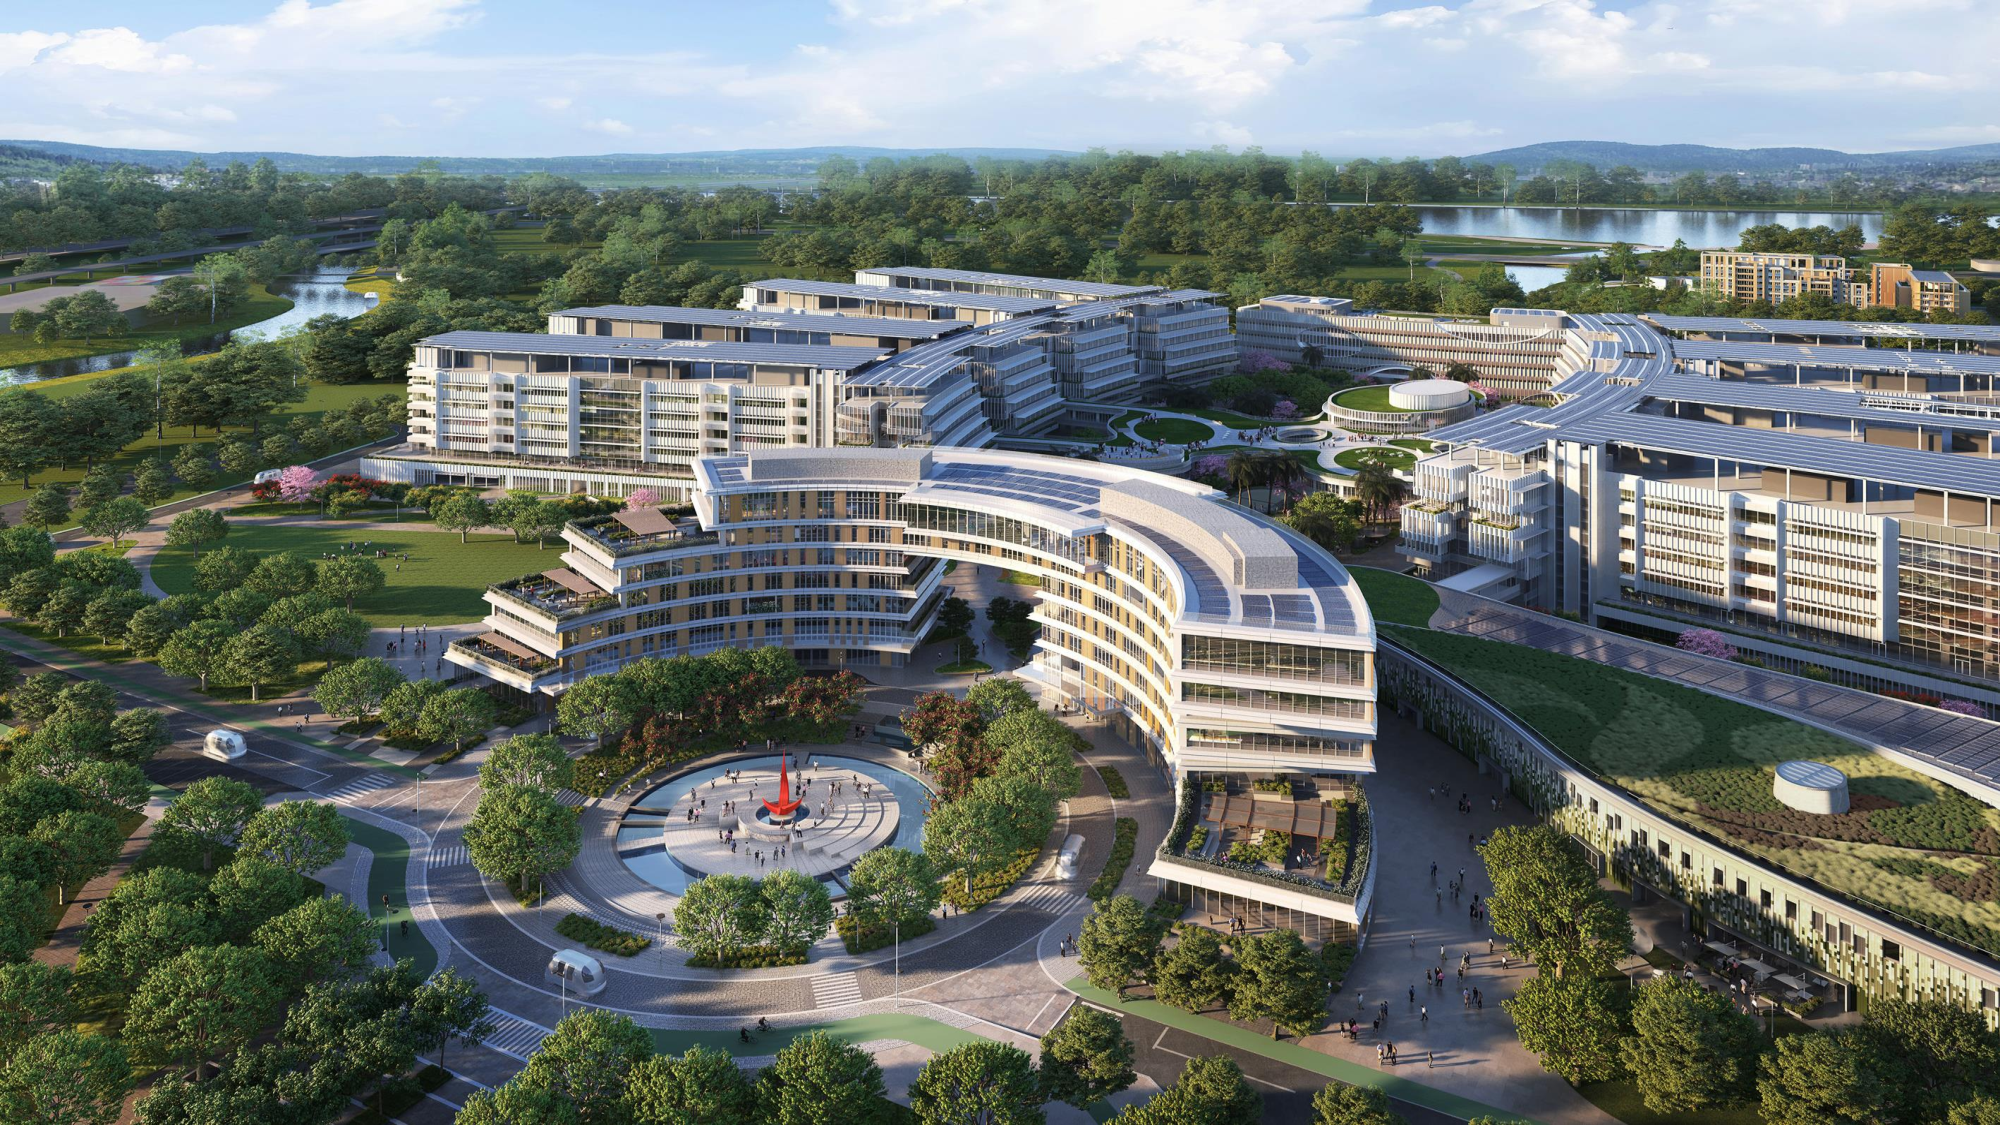
\includegraphics[
                width=\paperwidth,
                height=\paperheight]{figures/GZ Campus.jpeg}
        };
    \end{tikzpicture}
\end{frame}
}

% Outline
\AtBeginSection[]
{
    \begin{frame}[plain,noframenumbering]
        \frametitle{Outline}
        \begin{columns}[T]
            \begin{column}{0.01\textwidth}

            \end{column}
            \begin{column}{0.95\textwidth}
                \tableofcontents[currentsection,
                    %currentsubsection,
                    %hideothersubsections, 
                    %sectionstyle=show/sh ed, 
                    %subsectionstyle=show/shaded%/hide
                ]
            \end{column}
        \end{columns}
    \end{frame}
}

{ % title page
    \begin{frame}[plain]
        \maketitle
        \small
        \par\vskip-0.1em
        {\footnotesize
        \begin{beamercolorbox}[sep=8pt,left]{author}
            \usebeamerfont{author}{Presented by \insertauthor} on \insertdate
        \end{beamercolorbox}%\vskip0.5em
        }
        \note{
            Dear Professors, Dr. Li and Dr. Zhang, Good morning, given the group project, I will be presenting my individual topic. \\~\\

            I will start with the project overview.
        }

    \end{frame}
}
% % % % % % % % % % % % % % % % % % % % % % % % % % % % % % % % % % % %
\section{Introduction}
\subsection{Research Overview}
\begin{frame}
    \frametitle{Research Overview}
    \framesubtitle{Investigations on Deterministic and Probabilistic Forecasting}
    \begin{columns}
        \begin{column}{0.5\textwidth}
            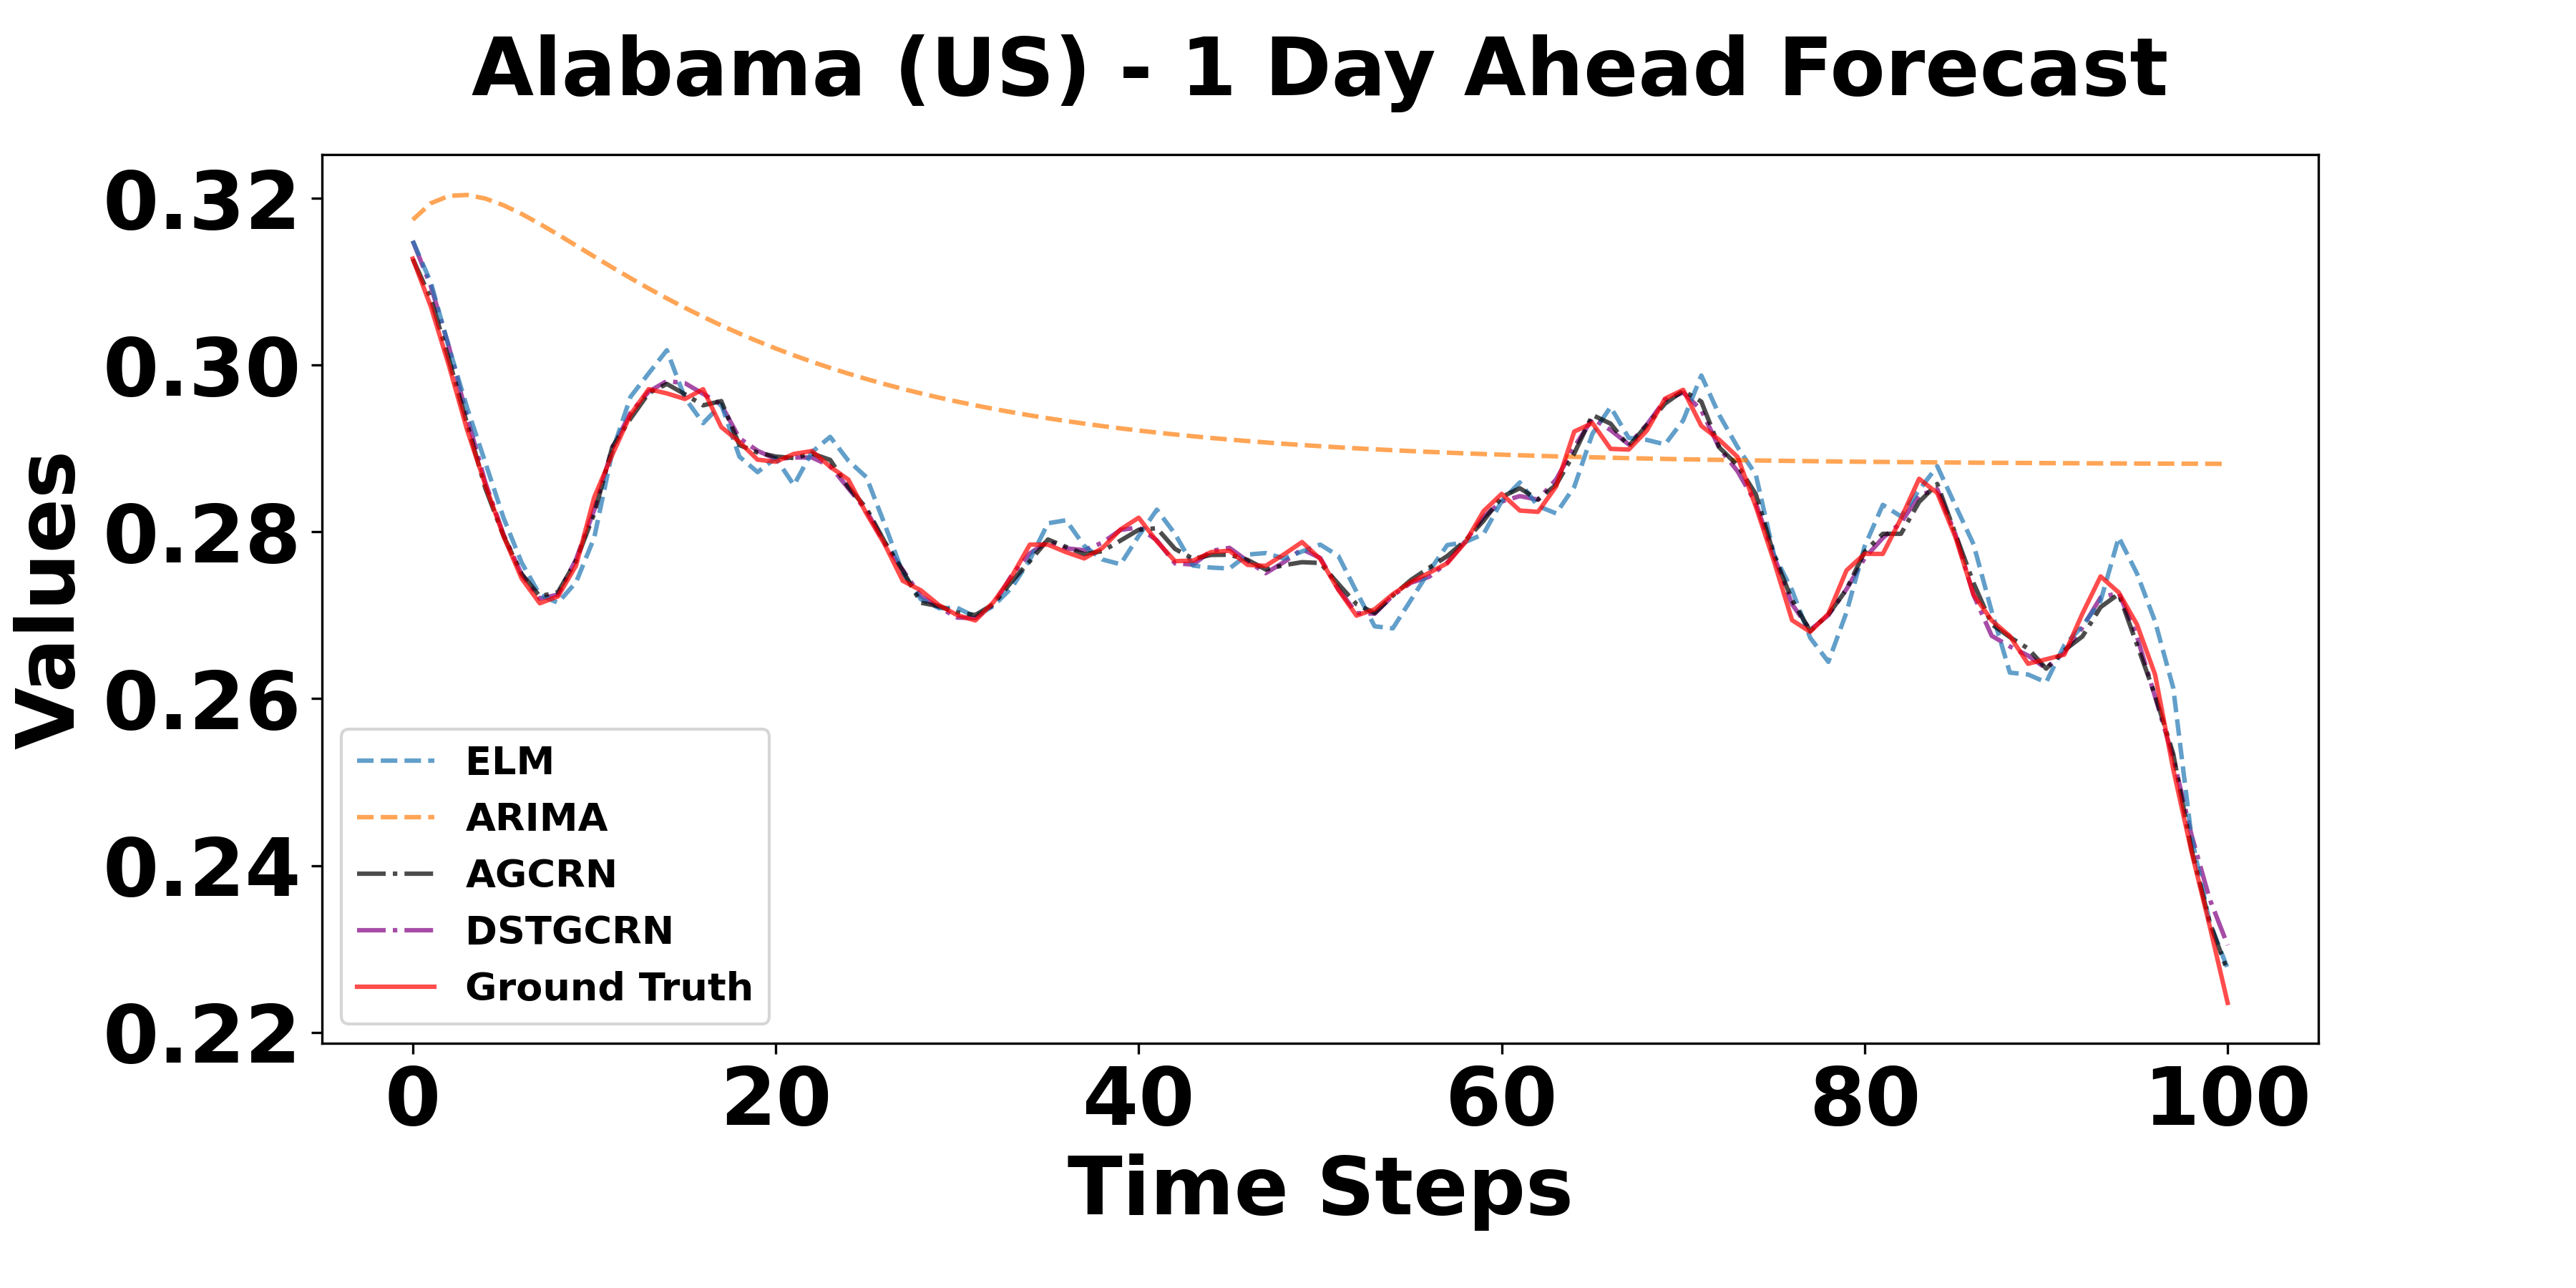
\includegraphics
            [width=\textwidth]{figures/1day_us_0region_modified_new.png}
            \captionof{figure}{A glimpse of forecasts comparison for deterministic carbon emissions forecasting}
        \end{column}
        \begin{column}{0.5\textwidth}
            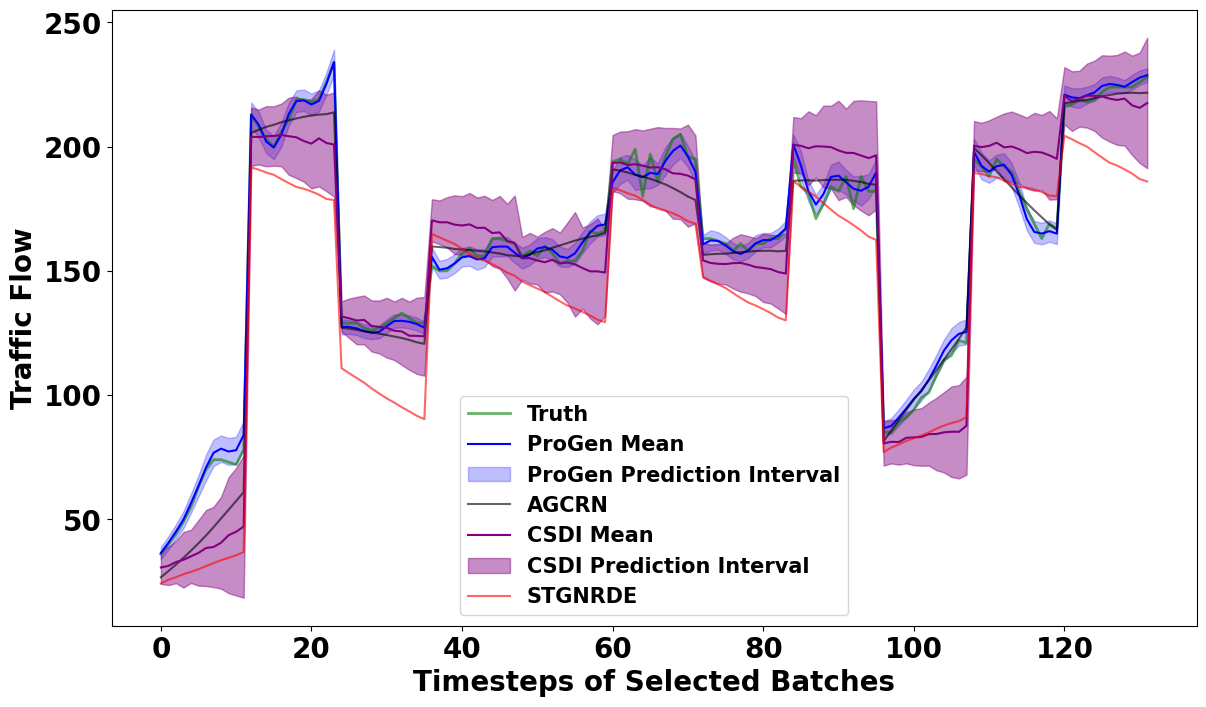
\includegraphics
            [width=\textwidth]{figures/node200_pems04.png}
            \captionof{figure}{A glimpse of forecasts comparison for probabilistic traffic flow forecasting}
        \end{column}
    \end{columns}
\end{frame}

% % % % % % % % % % % % % % % % % % % % % % % % % % % % % % % % % % % %

\section{Deterministic Carbon Emissions Modeling}
\subsection{Introduction}
\begin{frame}
    \frametitle{Introduction}
    \framesubtitle{DSTGCRN: Background and Motivation}
    \begin{columns}[T]
        \begin{column}{0.45\textwidth}
            \textbf{Background:}
            \begin{itemize}
                \item Sharp rise in human-driven carbon emissions from fossil fuels and land degradation.
                \item Crucial need for accurate emissions forecasting to:
                      \begin{itemize}
                          \item Support sustainable policies.
                          \item Achieve national reduction targets:
                                \begin{itemize}
                                    \item China: Peak by 2030.
                                    \item US: Reduce 50-52\% by 2030.
                                    \item EU: Cut 55\% by 2030.
                                \end{itemize}
                      \end{itemize}
            \end{itemize}
        \end{column}
        \begin{column}{0.45\textwidth}
            \textbf{Challenges:}
            \begin{itemize}
                \item Existing models miss non-linear trends and regional interdependencies.
                \item Key challenges in forecasting:
                      \begin{itemize}
                          \item Intra-region variability impacts overall emissions.
                          \item Inter-region dynamics affect regional emissions significantly.
                      \end{itemize}
            \end{itemize}
        \end{column}
    \end{columns}
\end{frame}


\begin{frame}
    \frametitle{Introduction}
    \framesubtitle{DSTGCRN: Motivations and Contributions}
    \begin{columns}[T] % Aligns the top of the content in both columns
        \begin{column}{0.45\textwidth}
            \textbf{Motivations:}
            \begin{itemize}
                \item Address complex and dynamic environmental data challenges overlooked by traditional methods.
                \item Inspired by the success of GNNs in related fields like traffic and energy, highlighting the need for advanced spatial-temporal analysis.
            \end{itemize}
        \end{column}
        \begin{column}{0.45\textwidth}
            \textbf{Contributions:}
            \begin{itemize}
                \item Integrates GCN and RNN to capture evolving inter-regional correlations and spatial-temporal interdependencies.
                \item Enhances predictive accuracy across multiple regions, offering detailed insights for environmental policy making.
                \item Supports strategic, real-time policymaking tailored to regional needs.
            \end{itemize}
        \end{column}
    \end{columns}
\end{frame}

\subsection{Literature Review}

\begin{frame}
    \frametitle{Literature Review}
    \framesubtitle{Statistical and Machine Learning Approaches}
    \begin{itemize}
        \item \textbf{Statistical Methods:}
              \begin{itemize}
                  \item ARIMA models are traditionally used for their capability to model and forecast time series data by identifying and adjusting for trends and seasonality.
                  \item Grey Forecasting Models (GM) are particularly useful in scenarios with limited or incomplete data, making them suitable for new or emerging markets.
                  \item Recent studies have combined GM with ARIMA to tackle both non-linear and non-stationary data features effectively, improving forecasting accuracy in complex scenarios.
              \end{itemize}
        \item \textbf{Machine Learning Methods:}
              \begin{itemize}
                  \item Neural networks, especially deep learning models, have shown superior performance due to their ability to learn complex patterns and interactions within large datasets.
                  \item These models are often integrated with traditional statistical methods to form hybrid models that leverage the strengths of both approaches, enhancing both accuracy and reliability of predictions.
                  \item Challenges include handling the diversity of regional environmental conditions, which can significantly impact model performance and scalability.
              \end{itemize}
    \end{itemize}
\end{frame}

\begin{frame}
    \frametitle{Literature Review}
    \framesubtitle{Advancements in Spatial-Temporal Predictions}
    \begin{itemize}
        \item \textbf{Developments:}
              \begin{itemize}
                  \item Spatial-Temporal Graph Neural Networks (STGNNs) are at the forefront of modeling complex interactions in time-dependent data across various locations, crucial for accurate environmental forecasting.
                  \item Innovations such as adaptive graph structures allow these models to dynamically adjust to changes in data over time, improving long-term prediction accuracy.
              \end{itemize}
        \item \textbf{Attention Mechanisms:}
              \begin{itemize}
                  \item Attention-based models have been developed to prioritize significant features and time steps, thus improving the focus on more impactful data points and reducing the noise from less relevant information.
                  \item These models have shown promising results in enhancing the granularity and specificity of environmental data analysis, addressing both spatial and temporal aspects effectively.
              \end{itemize}
    \end{itemize}
\end{frame}

\subsection{Methodology}

\begin{frame}
    \frametitle{Methodology Overview}
    \framesubtitle{Problem Definitions and Setup}
    \begin{itemize}
        \item \textbf{Multisource Time Series Forecasting:}
              Predict future values from multiple regional sources using observed data on various features like temperature and AQI.
              \[
                  \text{Forecast } \bm{Y}_{t+1}, \dots, \bm{Y}_{t+Q} \text{ using } f:\mathbb{R}^{N \times P \times C} \rightarrow \mathbb{R}^{N \times Q}
              \]
              where \( \bm{Y}_t \in \mathbb{R}^N \) is the output vector at time \( t \), \( P \) is the number of past time steps, and \( C \) is the number of features.

        \item \textbf{Regional Carbon Emission Network:}
              Uses a graph structure to model interdependencies among regions, enhancing prediction accuracy by incorporating spatial dynamics.
              \[
                  \mathcal{G} = (\mathcal{V}, \mathcal{E}, \bm{A}), \quad \bm{A}_{ij} =
                  \begin{cases}
                      1 & \text{if regions } i \text{ and } j \text{ are connected,} \\
                      0 & \text{otherwise.}
                  \end{cases}
              \]
              where \( \mathcal{V} \) represents the set of nodes (regions), \( \mathcal{E} \) represents the edges (connections between regions), and \( \bm{A} \) is the adjacency matrix.
    \end{itemize}
\end{frame}


\begin{frame}
    \frametitle{Adaptive Graph Convolutional Recurrent Network (AGCRN)}
    \framesubtitle{Core Modeling Approach}
    \begin{itemize}
        \item \textbf{Node Embedding and Graph Convolution:}
              \[
                  \bm{X}'_t = \left(\bm{I}_N + \text{softmax}\left(\text{ReLU}\left(\bm{E} \cdot \bm{E}^\top\right)\right)\right) \bm{X}_t \bm{\Theta}
              \]
              where \(\bm{I}_N\) is the identity matrix, \(\bm{\Theta}\) is the weight matrix.
        \item \textbf{Integration with GRU:}
              \begin{align*}
                  \tilde{\bm{A}} & = \text{softmax}(\text{ReLU}(\bm{E} \cdot \bm{E}^\top))                         \\
                  \bm{R}_t       & = \sigma(\tilde{\bm{A}}[\bm{X}_t, \bm{H}_{t-1}]\bm{E}\bm{W}_r + \bm{E}\bm{b}_r) \\
                  \bm{H}_t       & = \bm{R}_t \odot \bm{H}_{t-1} + (1 - \bm{R}_t) \odot \hat{\bm{H}}_t
              \end{align*}
        \item \textbf{Purpose:} Captures both spatial and temporal dependencies efficiently, integrating graph-based and sequence-based modeling.
    \end{itemize}
\end{frame}


\begin{frame}
    \frametitle{Methodology Detail}
    \framesubtitle{Dynamic Spatial-Temporal Modeling}
    \begin{itemize}
        \item \textbf{Dynamic Embeddings:}
              Generates dynamic node embeddings that adapt over time to capture evolving regional interdependencies. The embedding update mechanism is represented as:
              \[
                  \bm{E}_t = \text{DynamicEmbedding}(\bm{\mathcal{X}}_t), \quad \bm{\mathcal{X}}_t \in \mathbb{R}^{P \times N \times C}
              \]
              where \( \bm{\mathcal{X}}_t \) denotes the input features over \( P \) past time steps for \( N \) regions with \( C \) features each.

        \item \textbf{Multihead Attention:}
              Enhances the model's capability to discern distinct temporal patterns, significantly improving predictive accuracy. The multihead attention mechanism can be defined as:
              \[
                  \text{Attention}(\mathbf{Q}, \mathbf{K}, \mathbf{V}) = \text{softmax}\left(\frac{(\bm{\mathcal{X}}''_t \bm{W}_Q)(\bm{\mathcal{X}}''_t \bm{W}_K)^\top}{\sqrt{d_e}}\right)\bm{\mathcal{X}}''_t \bm{W}_V
              \]
              \begin{itemize}
                  \item \(\mathbf{Q}, \mathbf{K}, \mathbf{V}\) represent the queries, keys, and values, respectively, each transformed by distinct weight matrices \(\bm{W}_Q, \bm{W}_K, \bm{W}_V\).
                  \item \( \bm{\mathcal{X}}''_t \) is the input to the attention layer, and \( d_e \) is the dimension of the embedding space.
              \end{itemize}
    \end{itemize}
\end{frame}

\begin{frame}
    \frametitle{Dynamic Spatial-Temporal Modeling}
    \framesubtitle{Framework Visualization}
    \begin{figure}
        \centering
        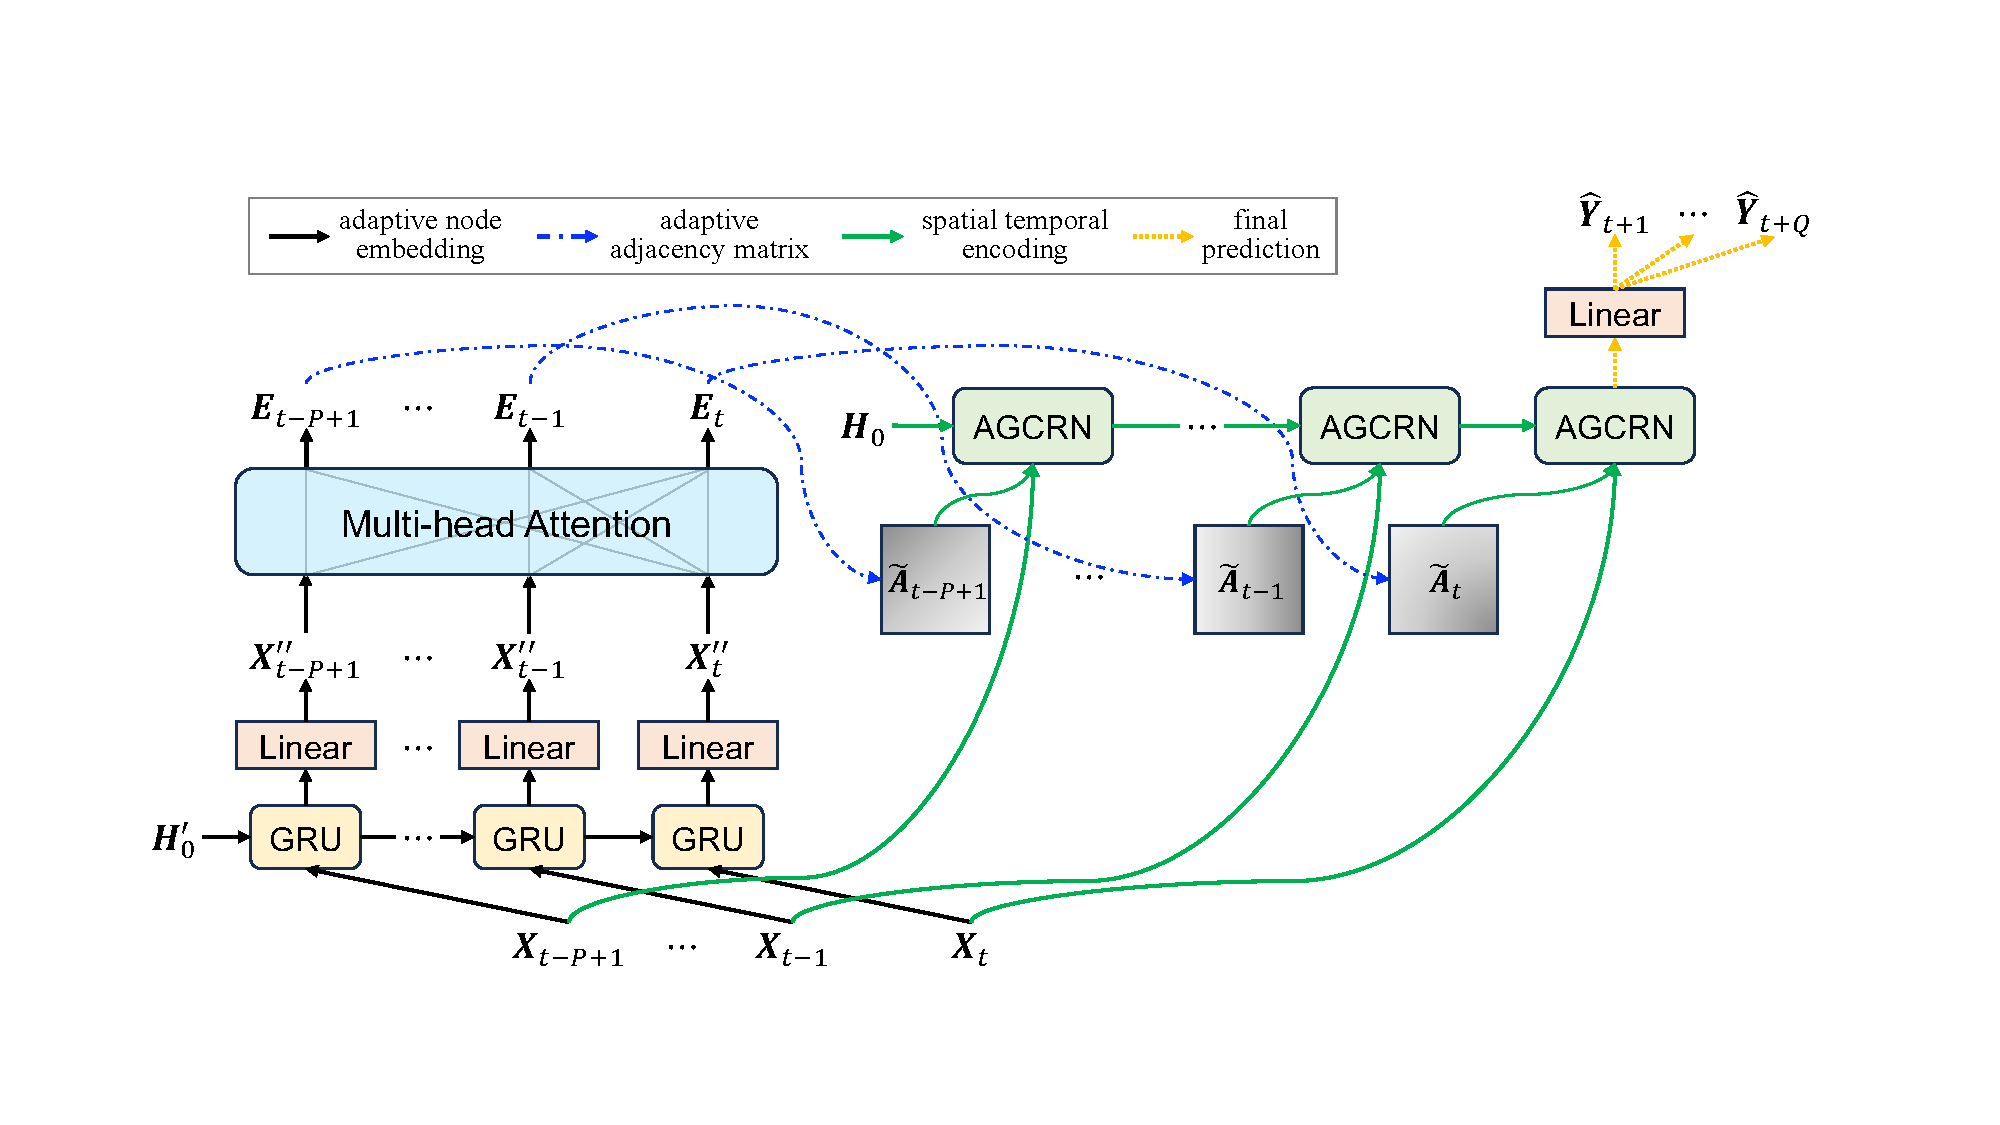
\includegraphics[width=0.8\textwidth]{figures/dstgcrn_framework.pdf}
        \caption{The architecture of the Dynamic Spatial-Temporal Graph Convolutional Recurrent Network (DSTGCRN).}
    \end{figure}
\end{frame}

\subsection{Results}

\begin{frame}
    \frametitle{Comparison of DSTGCRN Performance}
    \framesubtitle{Performance Across Datasets}
    \begin{figure}
        \centering
        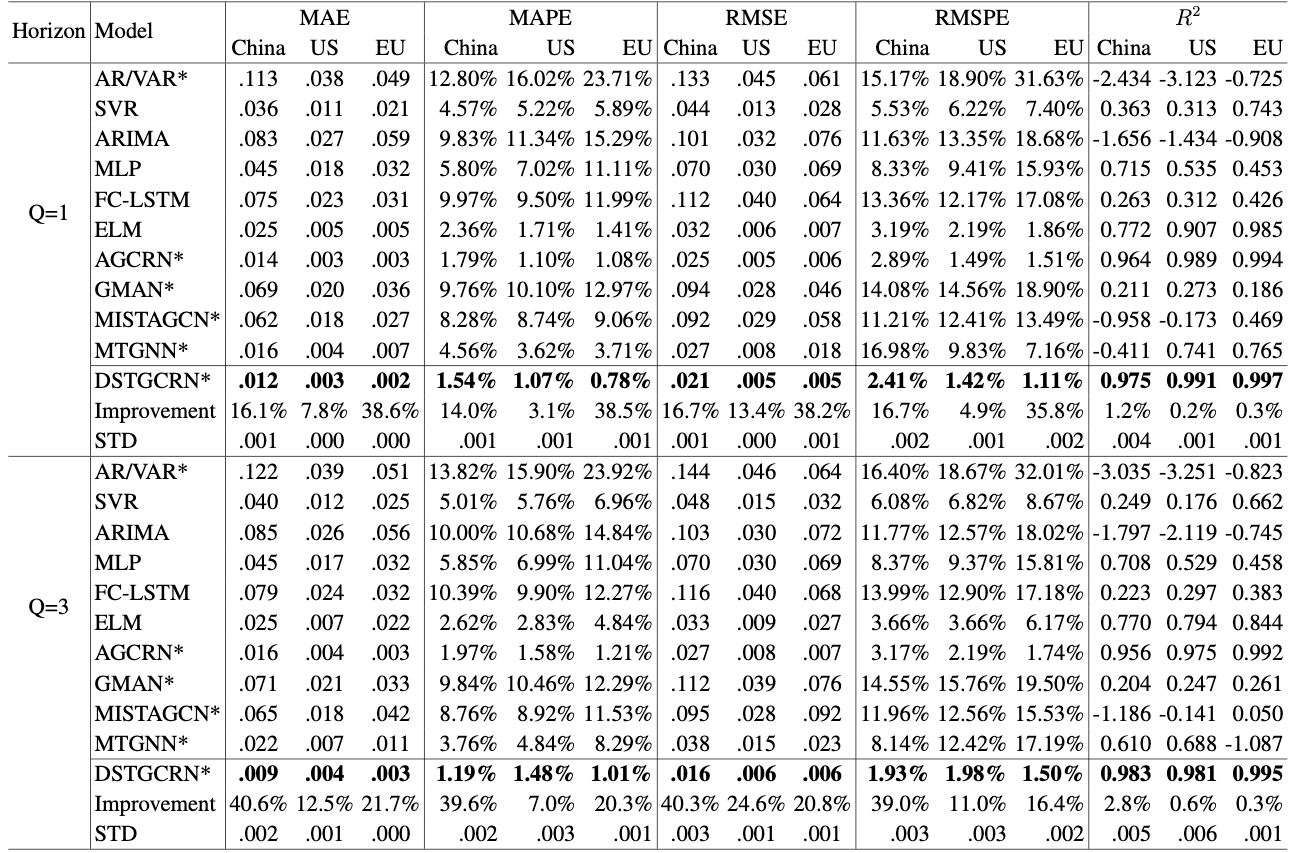
\includegraphics[width=0.6\textwidth]{figures/DSTGCRN_tab_results.png}
        \caption{Comparison of DSTGCRN with baselines after 5 runs on datasets from China, the US, and the EU. Models marked with an asterisk (*) also considered temperature and AQI data for China. Experiments used a 7-day lag, predicting 1 and 3 days ahead (Q=1, Q=3).}
    \end{figure}
\end{frame}



\begin{frame}
    \frametitle{Model Forecast Comparisons}
    \framesubtitle{Long Term Predictions}

    \begin{figure}
        \centering
        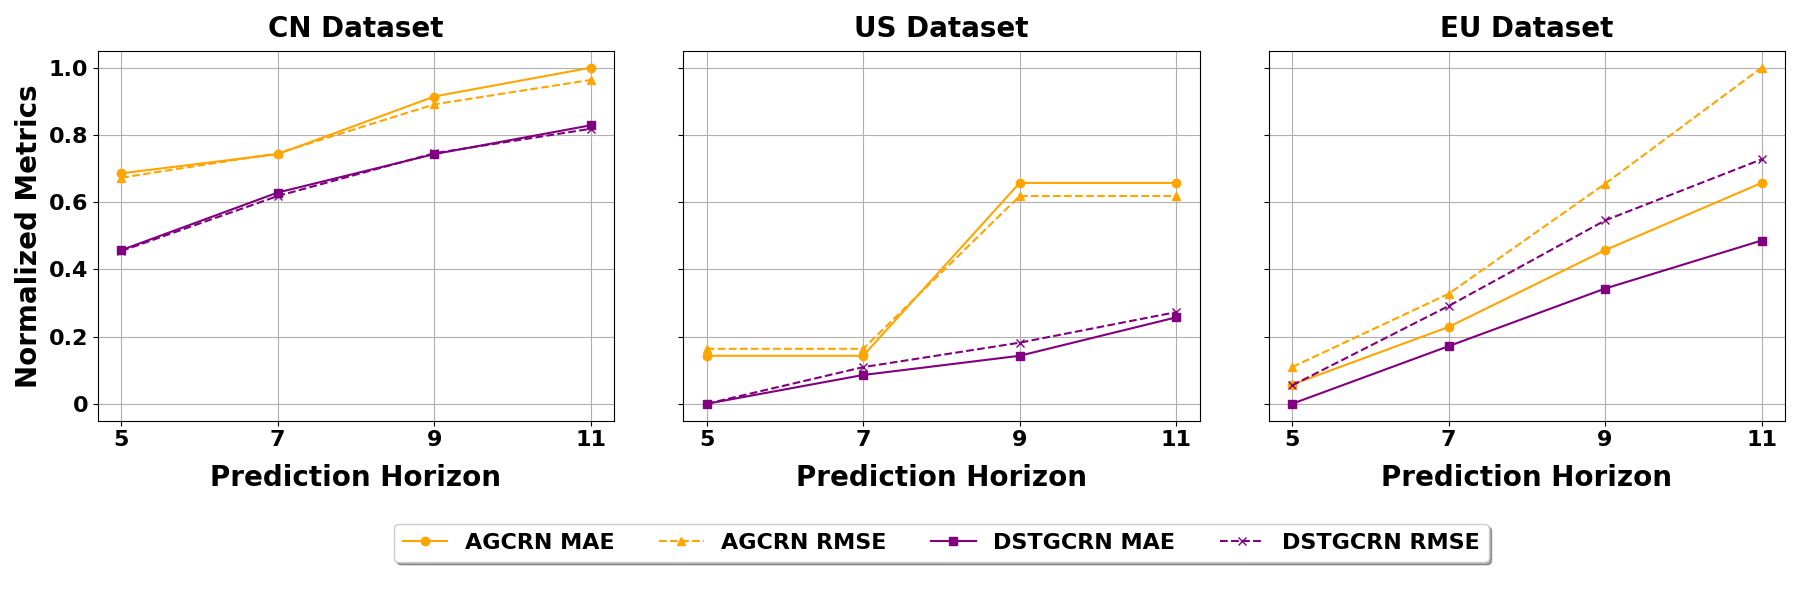
\includegraphics[width=\textwidth]{figures/longer_horizon.png}
        \caption{Performance comparison of AGCRN and DSTGCRN across geographies over longer horizons. This figure displays normalized MAE and RMSE metrics, enabling direct comparison on the same scale.}
    \end{figure}

\end{frame}

\begin{frame}
    \frametitle{Emission Trends and Model Comparisons}
    \framesubtitle{Visual Analysis of Data and Performance}

    \begin{columns}[T] % Top-aligned columns

        % Left column for the first figure
        \begin{column}{0.48\textwidth}
            \begin{figure}
                \centering
                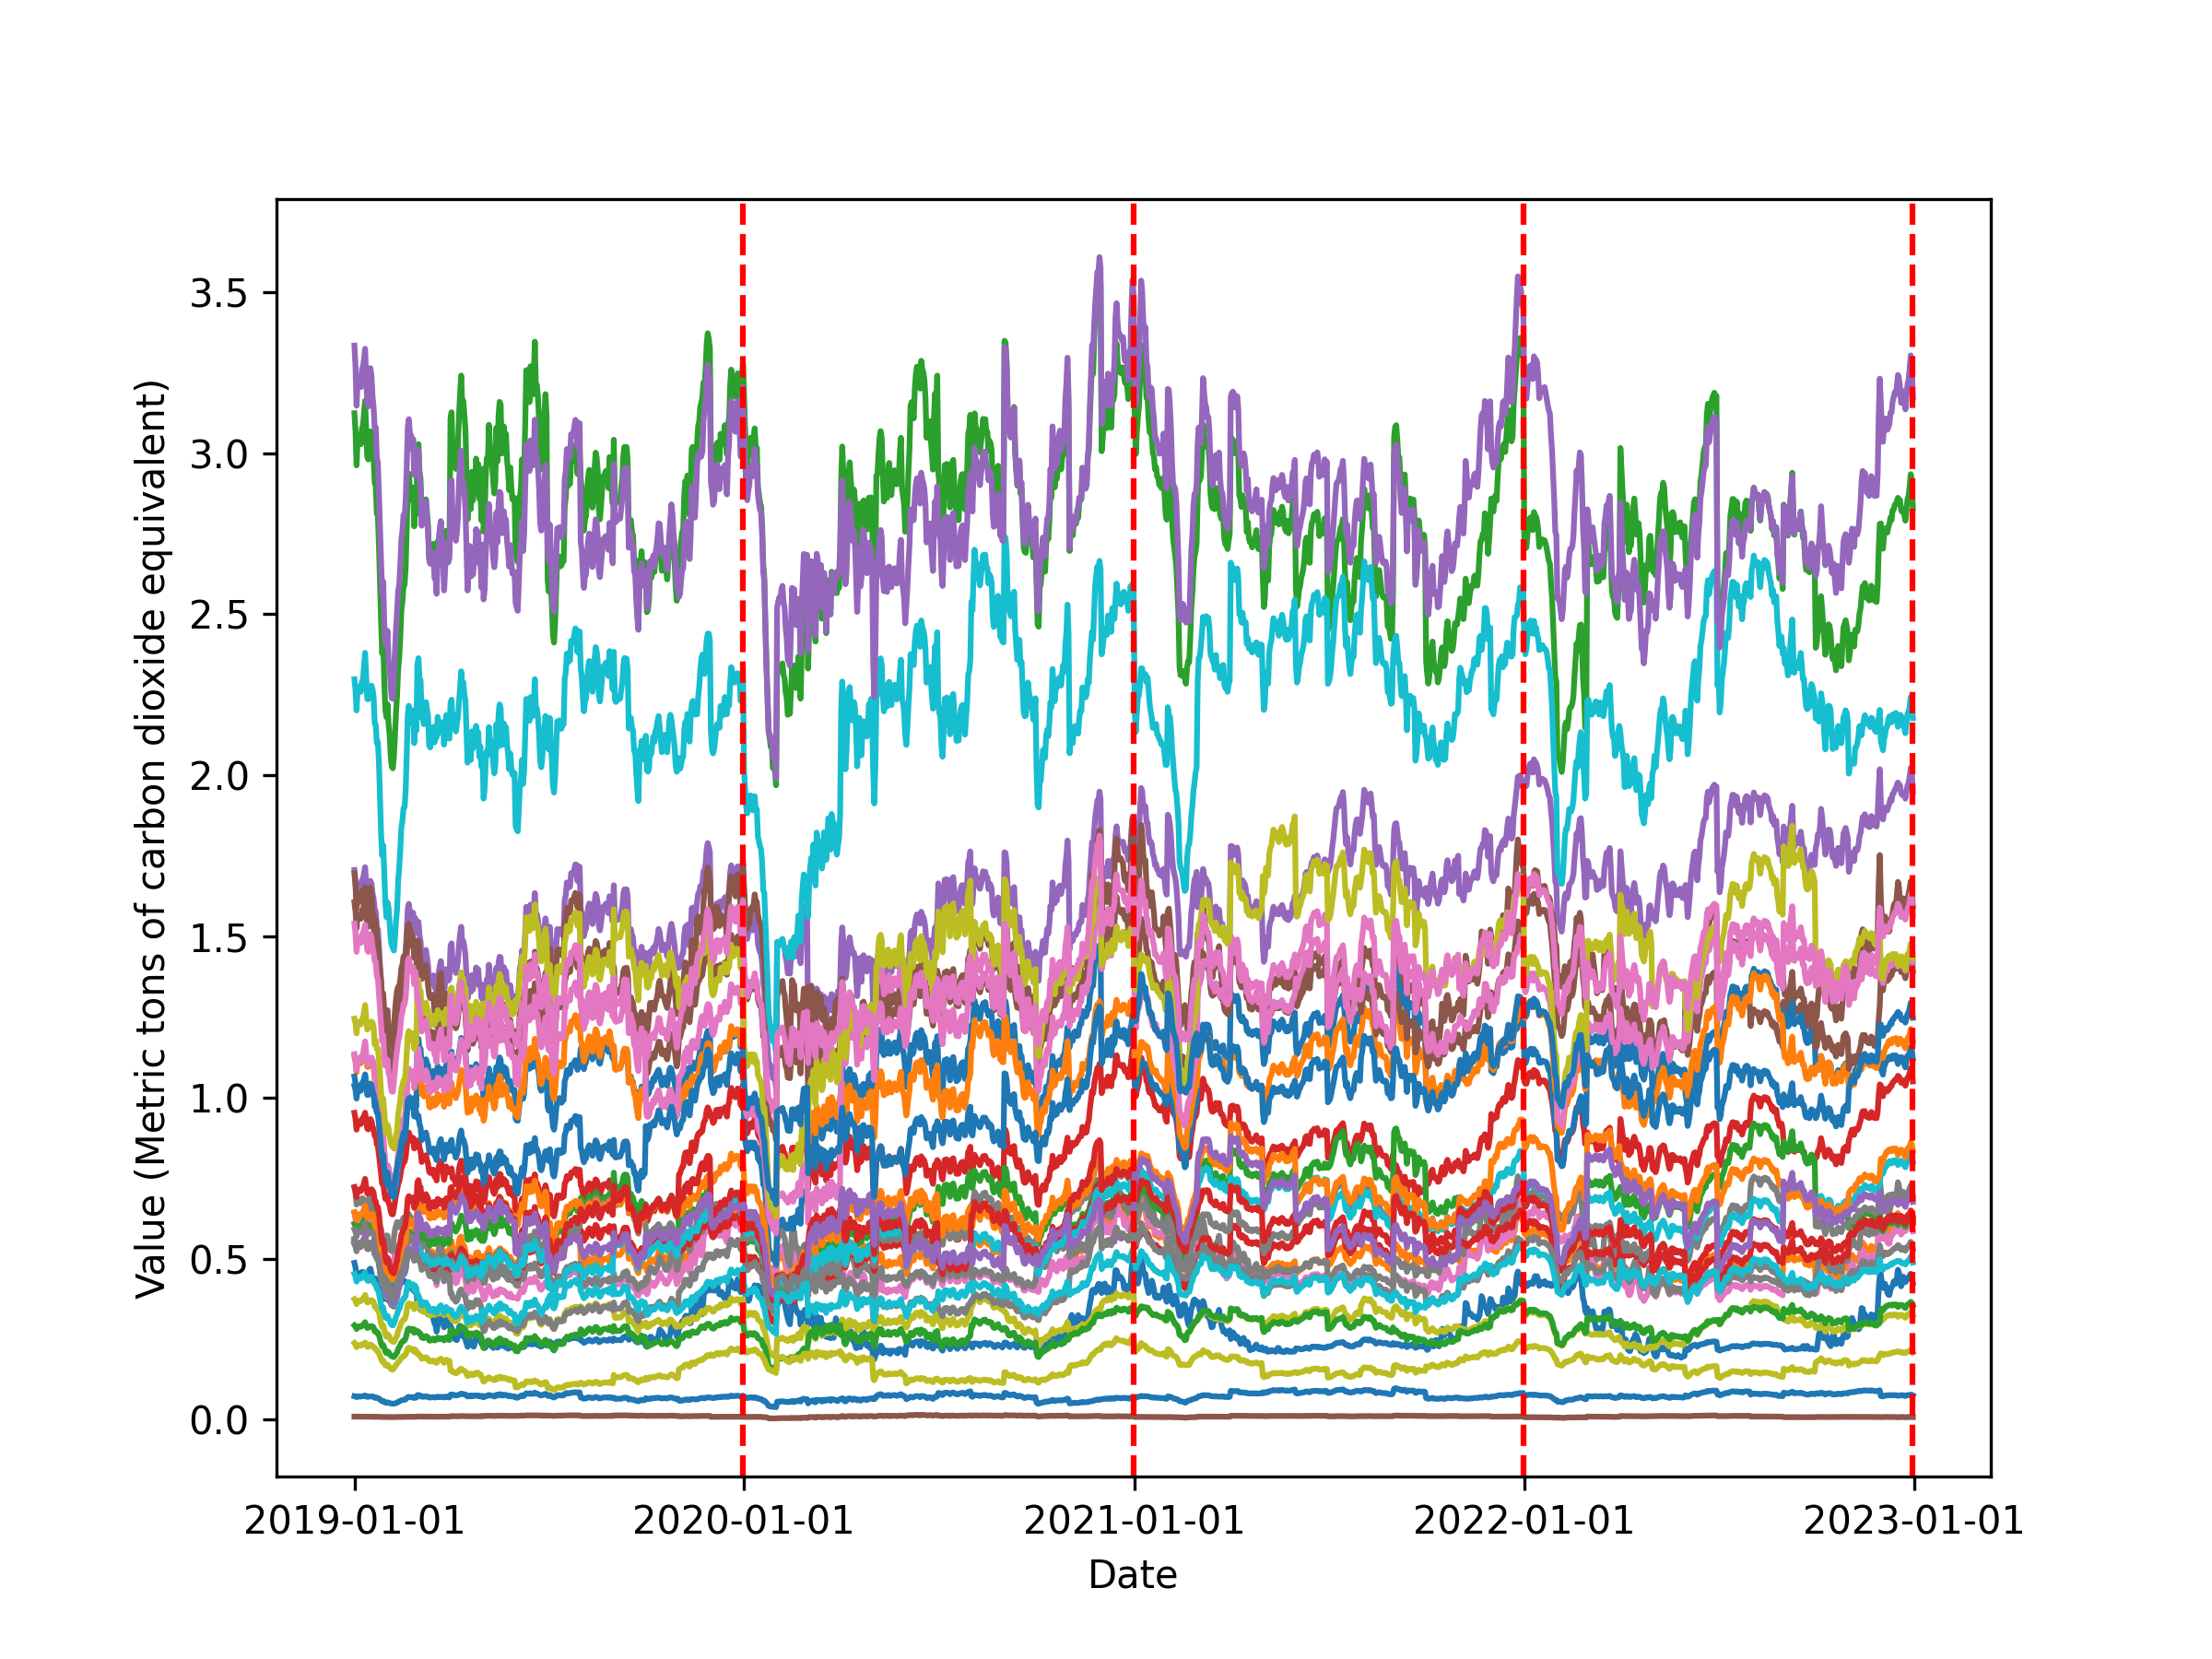
\includegraphics[width=\textwidth]{figures/combined_trend_plot.png}
                \caption{Provincial Carbon Emissions Trends from 2019 to 2022. Each color indicates the emission levels of individual provinces in China. Vertical dashed lines mark the commencement of each year.}
            \end{figure}
        \end{column}

        % Right column for the second figure
        \begin{column}{0.48\textwidth}
            \begin{figure}
                \centering
                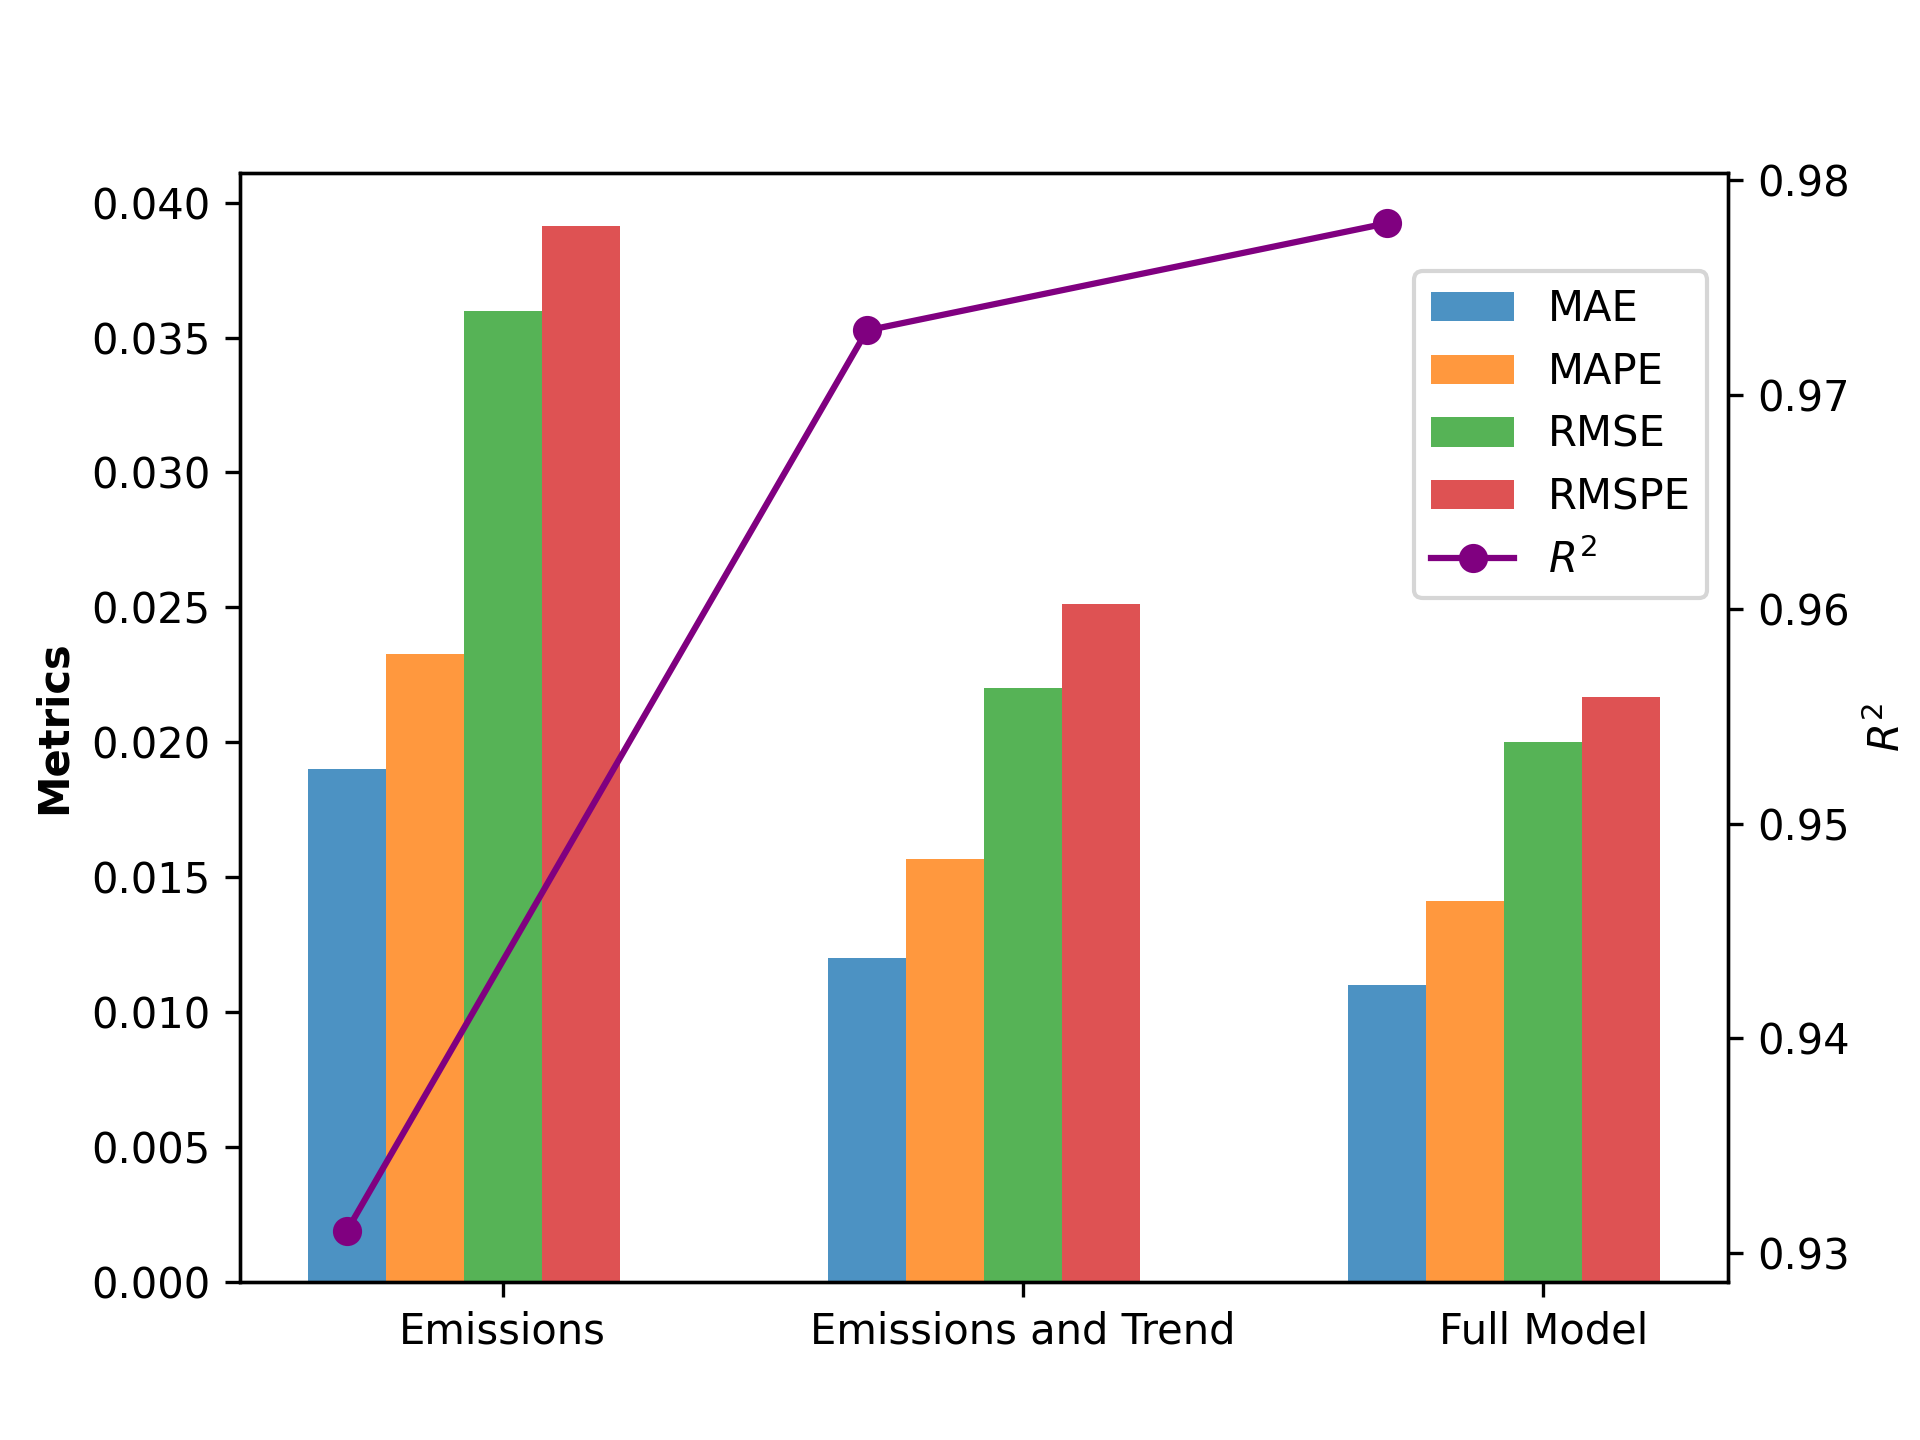
\includegraphics[width=\textwidth]{figures/comparison_feature.png}
                \caption{Comparison of model performance metrics across three predictive models.}
            \end{figure}
        \end{column}

    \end{columns}
\end{frame}

\begin{frame}
    \frametitle{Analysis of DSTGCRN}
    \framesubtitle{Matrix Evolution and Ablation Studies}

    \begin{columns}[T] % Top-aligned columns

        % Left column for the first figure
        \begin{column}{0.48\textwidth}
            \begin{figure}
                \centering
                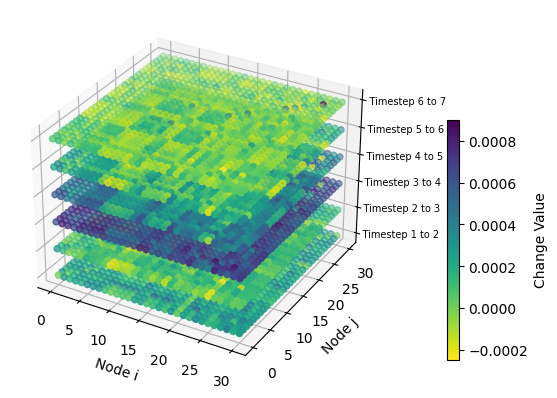
\includegraphics[width=\textwidth]{figures/adj_heatmap_stack.png}
                \caption{Differential Temporal Adjacency Matrix Evolution.}
            \end{figure}
        \end{column}

        % Right column for the second figure
        \begin{column}{0.48\textwidth}
            \begin{figure}
                \centering
                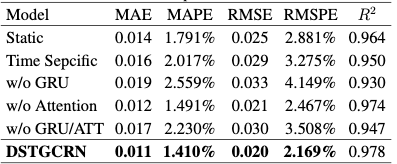
\includegraphics[width=\textwidth]{figures/dstgcrn_ablation.png}
                \caption{Ablation experiments on DSTGCRN.}
            \end{figure}
        \end{column}

    \end{columns}
\end{frame}

\section{Probabilistic Traffic Flow Forecasting}

\subsection{Introduction to ProGen}
\begin{frame}
    \frametitle{ProGen Framework}
    \framesubtitle{Background and Challenges}

    \begin{columns}[T]
        \begin{column}{0.48\textwidth}
            \textbf{Background:}
            \begin{itemize}
                \item Spatial-temporal data features complex spatial dependencies and dynamic temporal evolution.
                \item Traditional forecasting models often provide deterministic predictions that fail to capture inherent data uncertainties.
            \end{itemize}
        \end{column}
        \begin{column}{0.48\textwidth}
            \textbf{Challenges:}
            \begin{itemize}
                \item Difficulty in modeling the complex structures of spatial-temporal interactions.
                \item Existing deterministic models do not account for the probabilistic nature of real-world data, limiting their utility for decision-making.
            \end{itemize}
        \end{column}
    \end{columns}
\end{frame}


\begin{frame}
    \frametitle{ProGen Framework}
    \framesubtitle{Motivation and Contributions}

    \begin{columns}[T]
        \begin{column}{0.48\textwidth}
            \textbf{Motivation:}
            \begin{itemize}
                \item The rise of generative AI, particularly diffusion models, provides new tools for handling data uncertainty through probabilistic forecasts.
                \item ProGen utilizes stochastic differential equations (SDEs) to model the continuous-time evolution of data, enhancing forecasting accuracy.
            \end{itemize}
        \end{column}
        \begin{column}{0.48\textwidth}
            \textbf{Contributions:}
            \begin{itemize}
                \item \textbf{Conceptual:} A novel framework for continuous-time generative modeling for spatial-temporal forecasting.
                \item \textbf{Technical:} An innovative denoising network and tailored SDE that enhance handling of spatiotemporal correlations.
                \item \textbf{Empirical:} Demonstrated superiority over existing models through extensive validation on real-world datasets.
            \end{itemize}
        \end{column}
    \end{columns}
\end{frame}


\subsection{Literature Review}
\begin{frame}
    \frametitle{State of the Art in Probabilistic and Spatio-Temporal Forecasting}
    \framesubtitle{Diffusion Models, Probabilistic Forecasting, and Spatio-Temporal Methods}

    \begin{columns}[T]
        \begin{column}{0.48\textwidth}
            \textbf{Diffusion Models:}
            \begin{itemize}
                \item Pioneered by Ho et al. (2020) and Song et al. (2021), focusing on generating data from unconditioned noise through discrete and continuous SDEs.
                \item Extended to conditional generation for targeted outcomes, incorporating attributes to steer outputs (Nichol and Dhariwal 2021).
            \end{itemize}

            \textbf{Probabilistic Time Series Forecasting:}
            \begin{itemize}
                \item Adaptation of diffusion models for time series forecasting, like TimeGrad and ScoreGrad, faces challenges with autoregressive slow generation and accuracy in long-term forecasting (Shen and Kwok 2023).
                \item ProGen introduces a continuous approach for enhancing spatial and temporal correlation capture using SDEs.
            \end{itemize}
        \end{column}

        \begin{column}{0.48\textwidth}
            \textbf{Spatio-Temporal Forecasting:}
            \begin{itemize}
                \item Existing models like AGCRN and DSTAGNN use dynamic graphs for forecasting, while STG-NRDE utilizes neural rough differential equations.
                \item Discrete diffusion models have ventured into probabilistic forecasting but lack continuity in time series data handling, contrasting with ProGen's continuous-time approach (Wen et al. 2023).
            \end{itemize}
        \end{column}
    \end{columns}
\end{frame}

\subsection{Preliminaries}
\begin{frame}
    \frametitle{Probabilistic Spatio-Temporal Forecasting}
    \framesubtitle{Problem Setup}

    We aim to predict future values of a spatio-temporal series using historical data:
    \begin{itemize}
        \item Let \(\mathcal{D} = \{\mathbf{X_t}\}_{t=1}^T\) be a dataset where \(\mathbf{X_t} \in \mathbb{R}^{N \times D}\) represents observations at time \(t\), across \(N\) locations and \(D\) features.
        \item Spatial dependencies are encoded by a graph \(\mathcal{G} = (\mathcal{V}, \mathcal{E}, A)\), with nodes \(\mathcal{V}\), edges \(\mathcal{E}\), and adjacency matrix \(A\).
    \end{itemize}
    \begin{block}{Probabilistic Prediction Task}
        Estimate the distribution:
        \[
            q_X (\mathbf{X_{T+1:T+H}} \mid \mathbf{X_{T-L+1:T}}, \mathcal{G}, \mathcal{C})
        \]
        Here, \(L\) and \(H\) represent the historical window and forecasting horizon, respectively.
    \end{block}
\end{frame}


\begin{frame}
    \frametitle{Stochastic Differential Equations}
    \framesubtitle{Mathematical Foundation}

    SDEs provide a framework for modeling continuous-time stochastic processes:
    \begin{equation}
        d\mathbf{X} = f(\mathbf{X}, t)dt + g(\mathbf{X}, t)dW,
    \end{equation}
    where:
    \begin{itemize}
        \item \(\mathbf{X} \in \mathbb{R}^d\) represents the state at time \(t\).
        \item \(f(\mathbf{X}, t)\) is the drift function, dictating deterministic dynamics.
        \item \(g(\mathbf{X}, t)\) is the diffusion function, modeling stochastic effects.
        \item \(dW\) denotes differential Brownian motion.
    \end{itemize}
\end{frame}

\begin{frame}
    \frametitle{Reverse Stochastic Differential Equations}
    \framesubtitle{Retrieving Data from Noisy States}

    Reverse SDEs describe how to denoise data back to its original distribution:
    \begin{equation}
        d\mathbf{X} = \left[f(\mathbf{X}, t) - g^2(\mathbf{X}, t)\nabla_X \log p_t(\mathbf{X})\right]dt + g(\mathbf{X}, t)d\bar{W},
    \end{equation}
    \begin{itemize}
        \item The score function \(\nabla_X \log p_t(\mathbf{X})\) guides the denoising process.
        \item \(\bar{W}\) is the reverse Wiener process, introducing reverse dynamics.
    \end{itemize}
\end{frame}

\begin{frame}
    \frametitle{Denoising Score Matching (DSM)}
    \framesubtitle{Score-based Generative Modeling}

    DSM optimizes the match between the gradients of the log probabilities (scores) of the model and data distributions through the diffusion process:
    \begin{equation}
        \mathcal{L}(\theta) = \mathbb{E}_{t \sim \text{Uniform}(0, K)} \mathbb{E}_{X \sim p_{\text{data}}} [\|\nabla_X \log q_{\theta}(\mathbf{X^t} | t) - \nabla_X \log p_{\text{data}}(\mathbf{X^t} | t)\|^2]
    \end{equation}
    where:
    \begin{itemize}
        \item \( q_{\theta}(\mathbf{X^t} | t) \) and \( p_{\text{data}}(\mathbf{X^t} | t) \) are the model and data distributions at diffusion timestep \(t\), respectively.
        \item \( \nabla_X \log \) represents the gradient of the log probability.
        \item \( \theta \) denotes the model parameters optimized during training.
    \end{itemize}
\end{frame}

\begin{frame}
    \frametitle{Application of DSM and SDEs in ProGen}
    \framesubtitle{Practical Implementation and Forecasting Implications}

    ProGen's implementation of DSM and SDEs offers several key advantages for spatio-temporal forecasting:
    \begin{itemize}
        \item \textbf{Improved Forecast Accuracy:} By accounting for uncertainty and enabling the model to explore a range of possible futures.
        \item \textbf{Robustness to Noise:} The use of SDEs helps handle the inherent noise and variability in spatio-temporal data effectively.
        \item \textbf{Flexibility in Model Application:} Suitable for various types of spatio-temporal data beyond just traffic or weather, including economic and biological datasets.
    \end{itemize}
    Additionally, the continuous-time approach of ProGen allows for finer temporal resolution in predictions, crucial for dynamic systems monitoring and decision-making.
\end{frame}

\subsection{Methodology}
\begin{frame}
    \frametitle{Overview of ProGen Framework}
    \framesubtitle{Operational Processes}

    ProGen combines a forward diffusion process with a reverse prediction process:
    \begin{itemize}
        \item \textbf{Forward Diffusion:} Transforms training data into a Gaussian state while training a score model.
        \item \textbf{Reverse Prediction:} Iteratively denoises to generate predictions, guided by the score model.
    \end{itemize}

    \begin{figure}[ht]
        \centering
        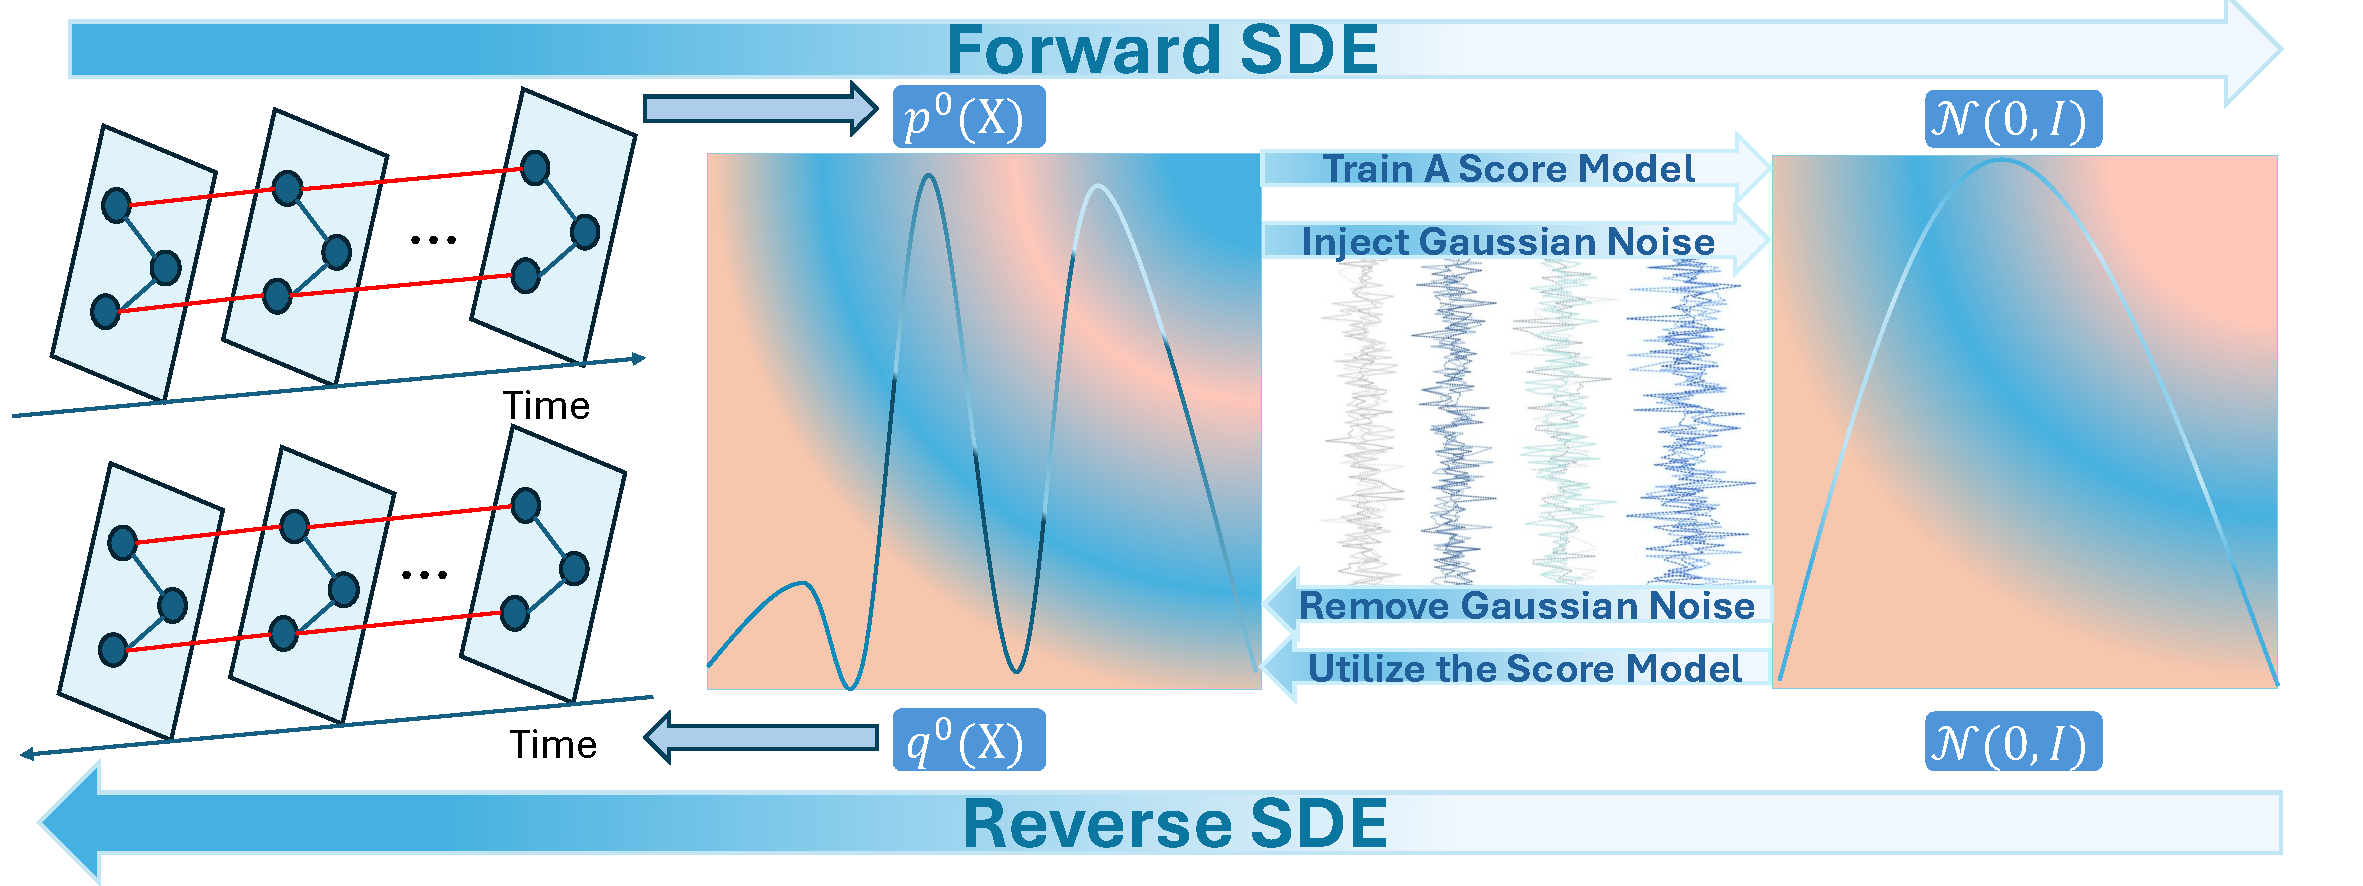
\includegraphics[width=0.7\textwidth]{figures/ProGen_framework_new.pdf}
        \caption{Overview of the two primary processes in ProGen.}
        \label{fig:framework}
    \end{figure}

\end{frame}

\begin{frame}
    \frametitle{Forward Diffusion Process}
    \framesubtitle{Transforming Data into Gaussian State}

    The forward process perturbs the data point by point into Gaussian noise:
    \begin{equation}
        \mathbf{\tilde{X}^t_{F}} = \mu(\mathbf{X_{F}}, t) + \sigma(\mathbf{X_{F}}, t) \times Z, \quad Z \sim \mathcal{N}(0, I)
    \end{equation}
    where \(\mu\) and \(\sigma\) control the mean and standard deviation across discretized time steps.

    This process trains the model to understand and simulate the transition from real data distributions to noise.
\end{frame}

\begin{frame}
    \frametitle{Training the Denoising Score Model}
    \framesubtitle{Optimizing the Score Estimation}

    Training focuses on minimizing the discrepancy between the estimated and true data gradients:
    \begin{equation}
        \mathcal{L}(\theta) = \mathbb{E}_{t} \left\{ \mathbb{E}_{\mathbf{X}_{F}, \mathbf{X_H}} \left[ \|\nabla \log p(\tilde{\mathbf{X}}_{F}^t | \mathbf{X}_{F}) - s_\theta(\tilde{\mathbf{X}}_{F}^t, \mathbf{X_H})\|^2 \right] \right\}
    \end{equation}
    This loss function aligns the model's score estimates with the true distribution changes, enhancing prediction accuracy.

    \begin{figure}[ht]
        \centering
        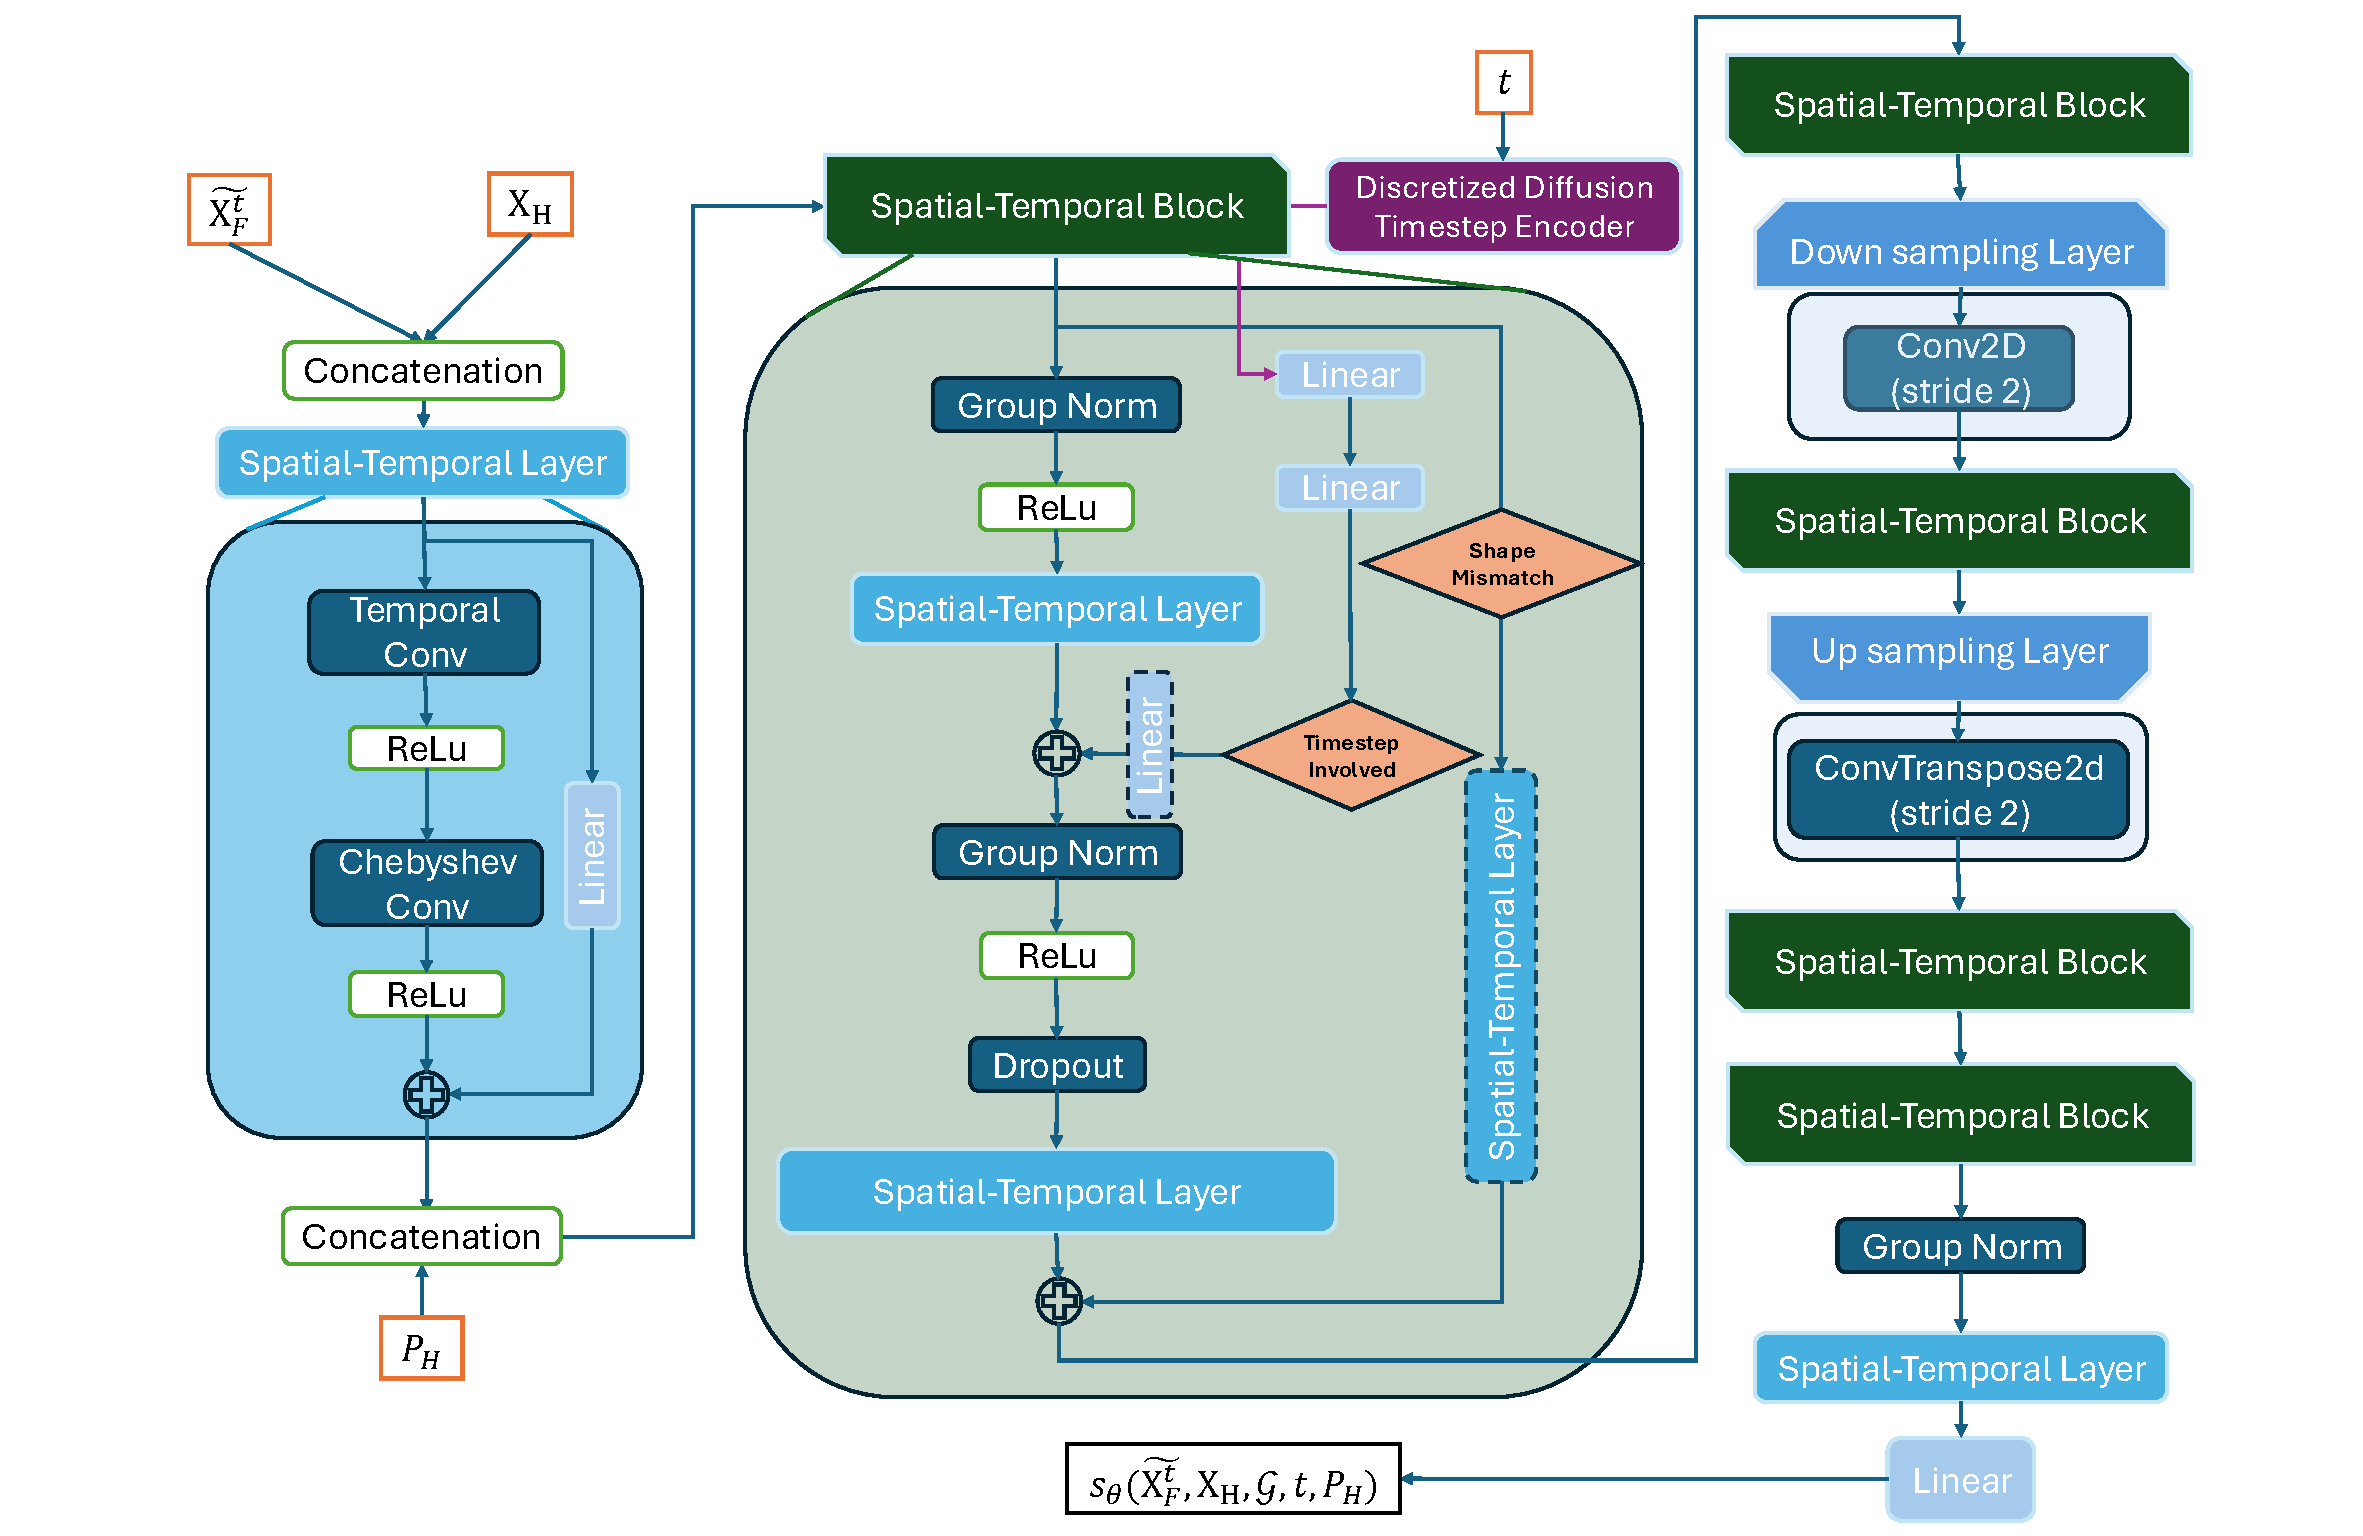
\includegraphics[width=0.75\textwidth]{figures/ProGen_model.pdf}
        \caption{Architecture of the Denoising Score Matching Model in ProGen.}
        \label{fig:model}
    \end{figure}

\end{frame}

\begin{frame}
    \frametitle{Adaptive Reverse Prediction Process}
    \framesubtitle{Restoring Original Data Distribution}

    The reverse SDE effectively restores data from its noisy state using learned scores:
    \begin{equation}
        d\mathbf{X} = (f(\mathbf{X}, t) - g(\mathbf{X}, t)^2 \nabla \log p(\mathbf{X}|t))dt + g(\mathbf{X}, t)d\bar{W}
    \end{equation}
    This equation integrates insights from the score model to reverse the diffusion, guiding the data back to its original state.

    ProGen's approach modifies traditional methods by adapting to data dynamics more effectively and efficiently.
\end{frame}

\subsection{Results}
\begin{frame}
    \frametitle{Overview of ProGen Performance}
    \framesubtitle{Full Test Run}

    \begin{figure}[ht]
        \centering
        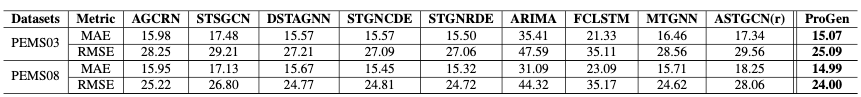
\includegraphics[width=\textwidth]{figures/det_full_tab.png}
        \caption{Distribution and mean values of predictions vs. actual truths across initial batch iterations in PEMS04.}
    \end{figure}

    \begin{figure}[htbp]
        \centering
        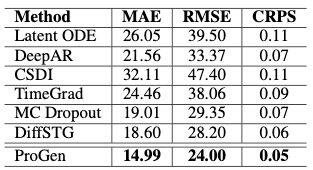
\includegraphics[width=0.35\textwidth]{figures/prob_full_tab.png}
        \caption{Training loss curves for different spatiotemporal layers in PEMS08 over 100 epochs.}
    \end{figure}
\end{frame}

\begin{frame}
    \frametitle{Overview of ProGen Performance}
    \framesubtitle{Random Test Runs}

    \begin{figure}[ht]
        \centering
        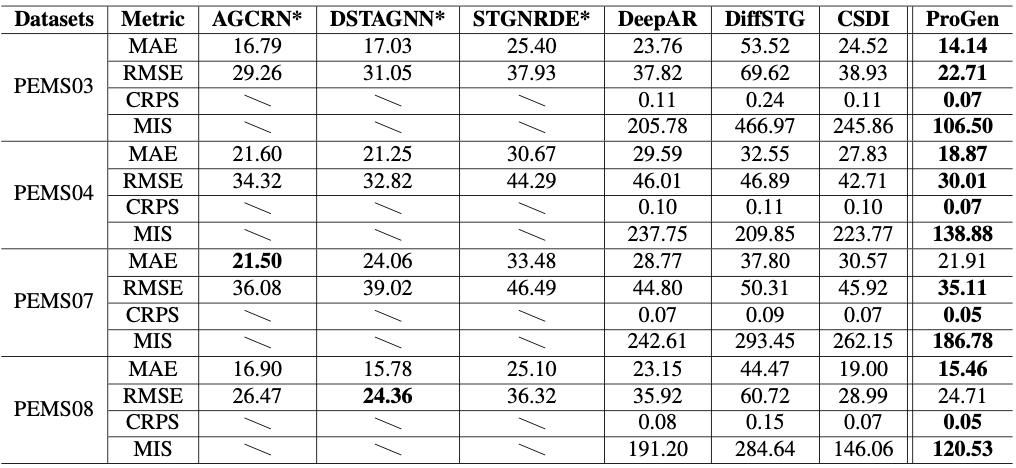
\includegraphics[width=0.8\textwidth]{figures/random_runs_tab.png}
        \caption{Distribution and mean values of predictions vs. actual truths across initial batch iterations in PEMS04.}
    \end{figure}
\end{frame}


\begin{frame}
    \frametitle{Overview of ProGen Performance}
    \framesubtitle{Random Test Runs}

    \begin{figure}[ht]
        \centering
        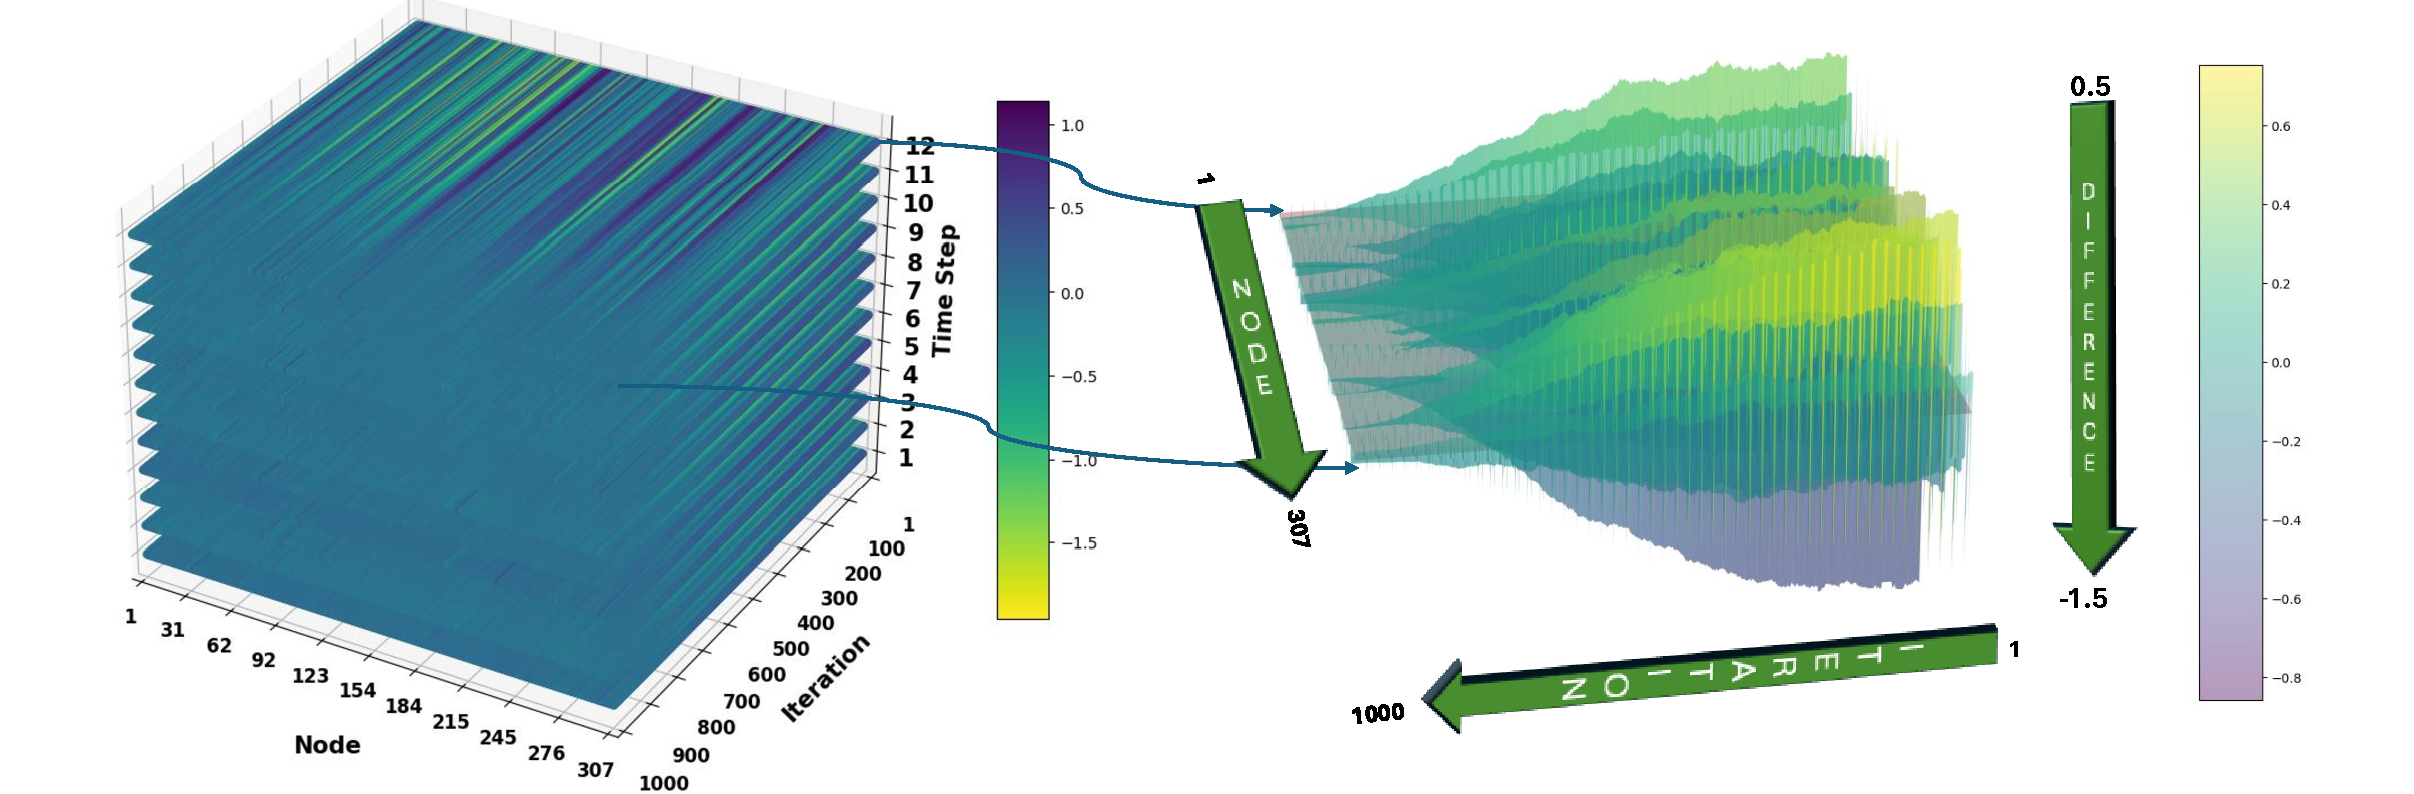
\includegraphics[width=0.8\textwidth]{figures/pems04_3d_waves_plot.pdf}
        \caption{Distribution and mean values of predictions vs. actual truths across initial batch iterations in PEMS04.}
    \end{figure}
\end{frame}



\begin{frame}
    \frametitle{Overview of ProGen Performance}
    \framesubtitle{Random Test Runs}

    \begin{figure}[ht]
        \centering
        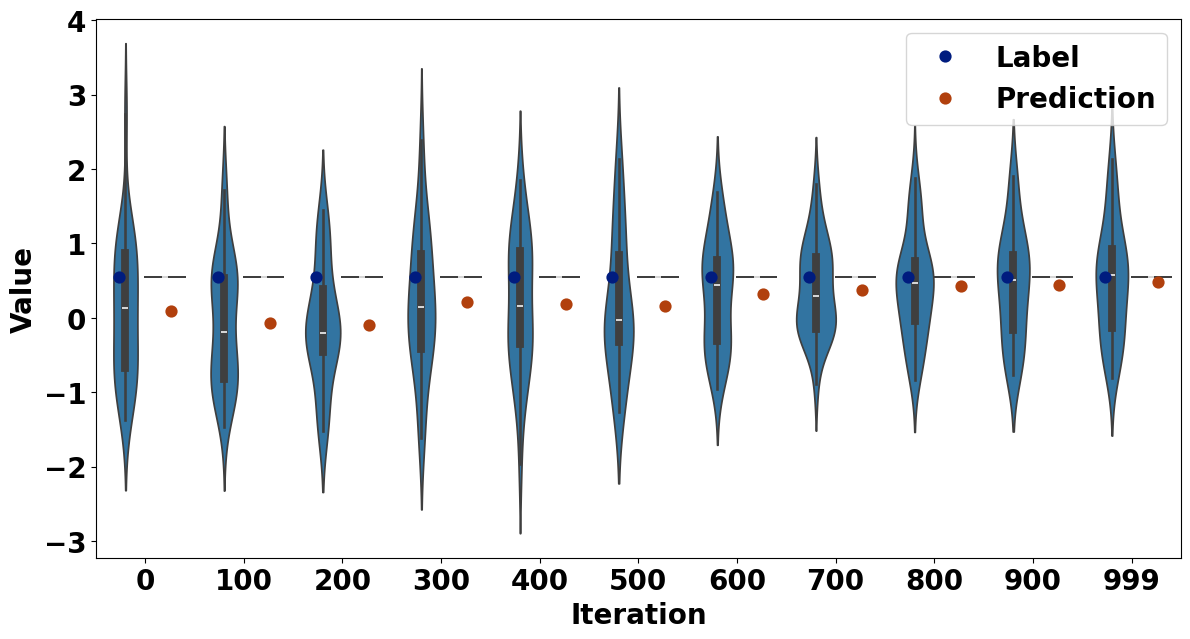
\includegraphics[width=0.8\textwidth]{figures/distribution_change_iteration_pems04.png        }
        \caption{Distribution and mean values of predictions vs. actual truths across initial batch iterations in PEMS04.}
    \end{figure}
\end{frame}


\begin{frame}
    \frametitle{Overview of ProGen Performance}
    \framesubtitle{Random Test Runs}

    \begin{figure}[ht]
        \centering
        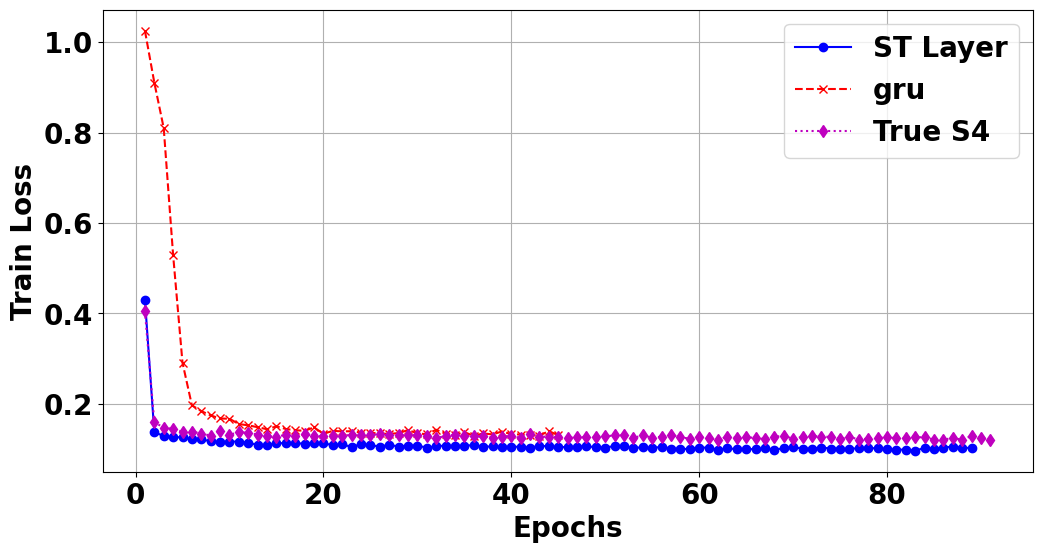
\includegraphics[width=0.8\textwidth]{figures/train_loss.png        }
        \caption{Distribution and mean values of predictions vs. actual truths across initial batch iterations in PEMS04.}
    \end{figure}
\end{frame}

\begin{frame}
    \frametitle{Overview of ProGen Performance}
    \framesubtitle{Random Test Runs}

    \begin{figure}[ht]
        \centering
        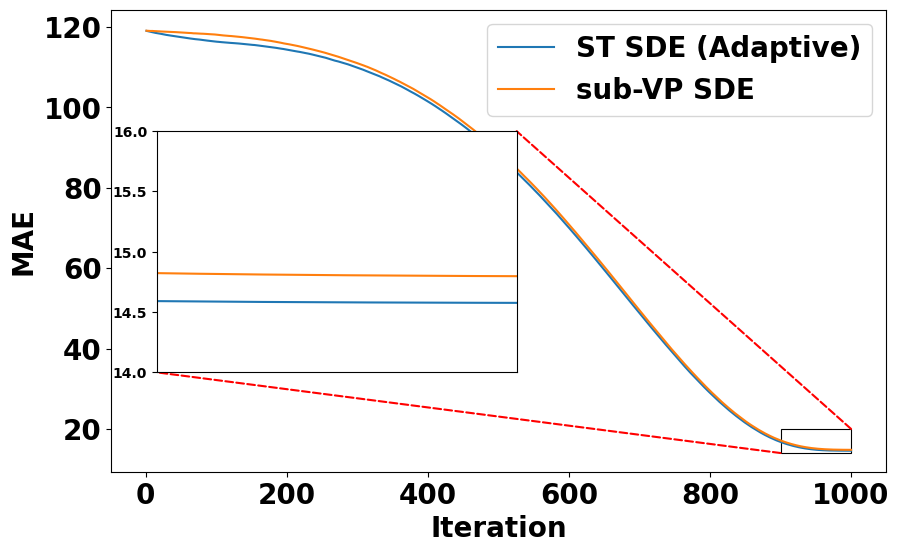
\includegraphics[width=0.8\textwidth]{figures/mae_stsde_subvpsde.png        }
        \caption{Distribution and mean values of predictions vs. actual truths across initial batch iterations in PEMS04.}
    \end{figure}
\end{frame}

\begin{frame}
    \frametitle{Overview of ProGen Performance}
    \framesubtitle{Random Test Runs}

    \begin{figure}[ht]
        \centering
        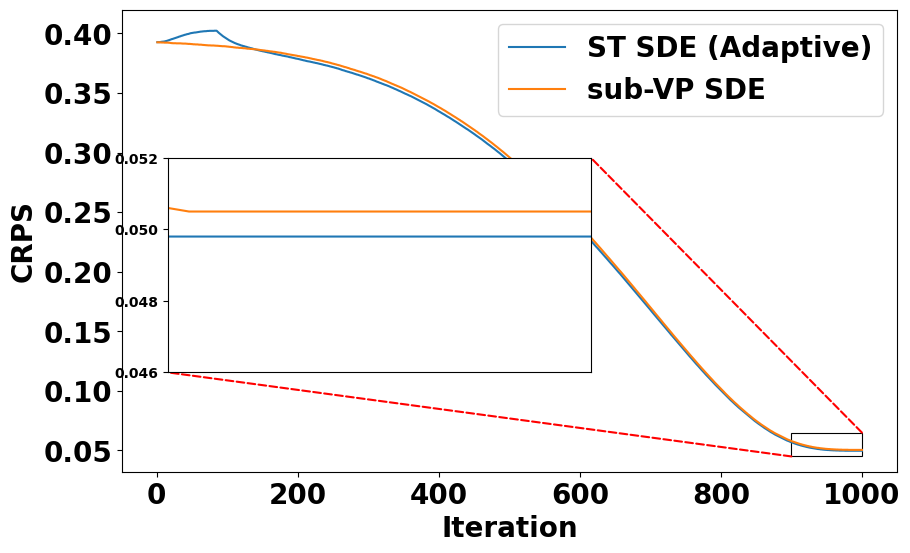
\includegraphics[width=0.8\textwidth]{figures/crps_stsde_subvpsde.png        }
        \caption{Distribution and mean values of predictions vs. actual truths across initial batch iterations in PEMS04.}
    \end{figure}
\end{frame}

\begin{frame}
    \frametitle{Overview of ProGen Performance}
    \framesubtitle{Random Test Runs}

    \begin{figure}[ht]
        \centering
        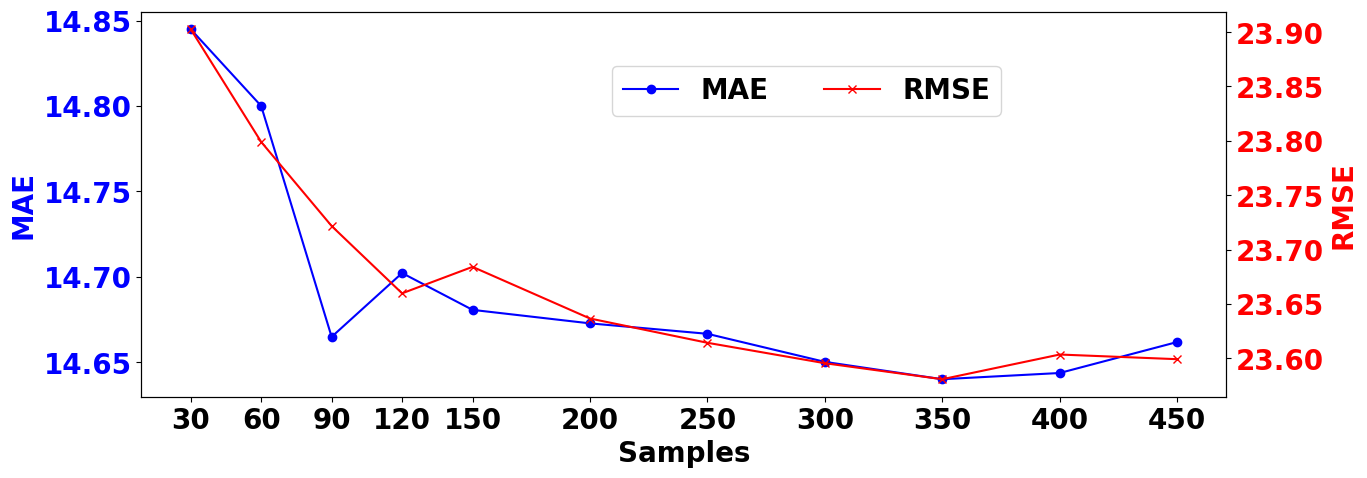
\includegraphics[width=0.8\textwidth]{figures/mae_rmse_samples.png       }
        \caption{Distribution and mean values of predictions vs. actual truths across initial batch iterations in PEMS04.}
    \end{figure}
\end{frame}

\begin{frame}
    \frametitle{Overview of ProGen Performance}
    \framesubtitle{Random Test Runs}

    \begin{figure}[ht]
        \centering
        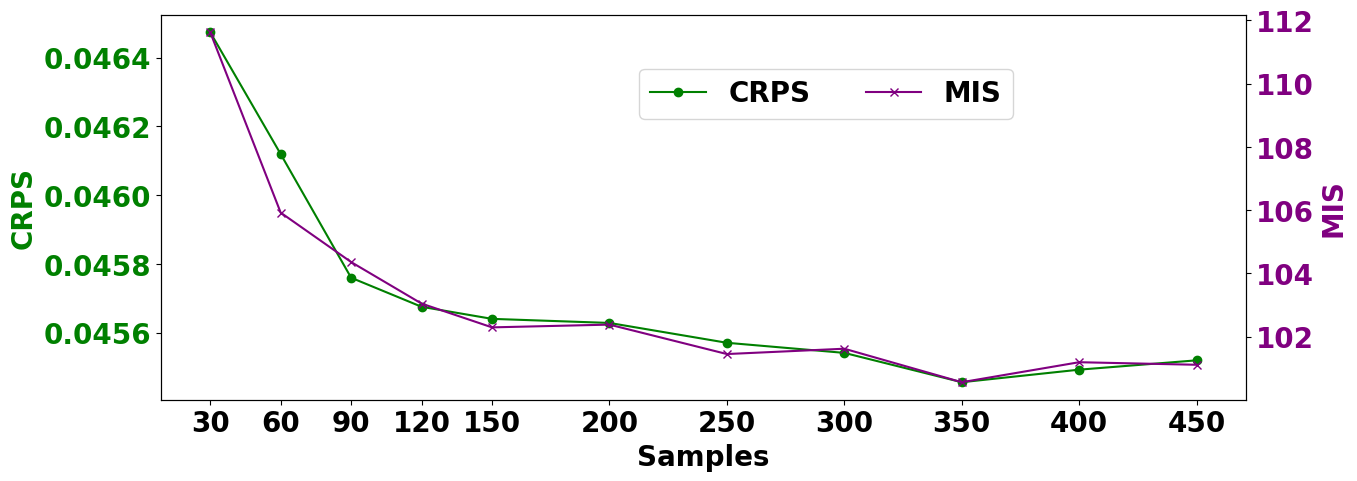
\includegraphics[width=0.8\textwidth]{figures/crps_mis_samples.png        }
        \caption{Distribution and mean values of predictions vs. actual truths across initial batch iterations in PEMS04.}
    \end{figure}
\end{frame}

\begin{frame}
    \frametitle{Overview of ProGen Performance}
    \framesubtitle{Random Test Runs}

    \begin{figure}[ht]
        \centering
        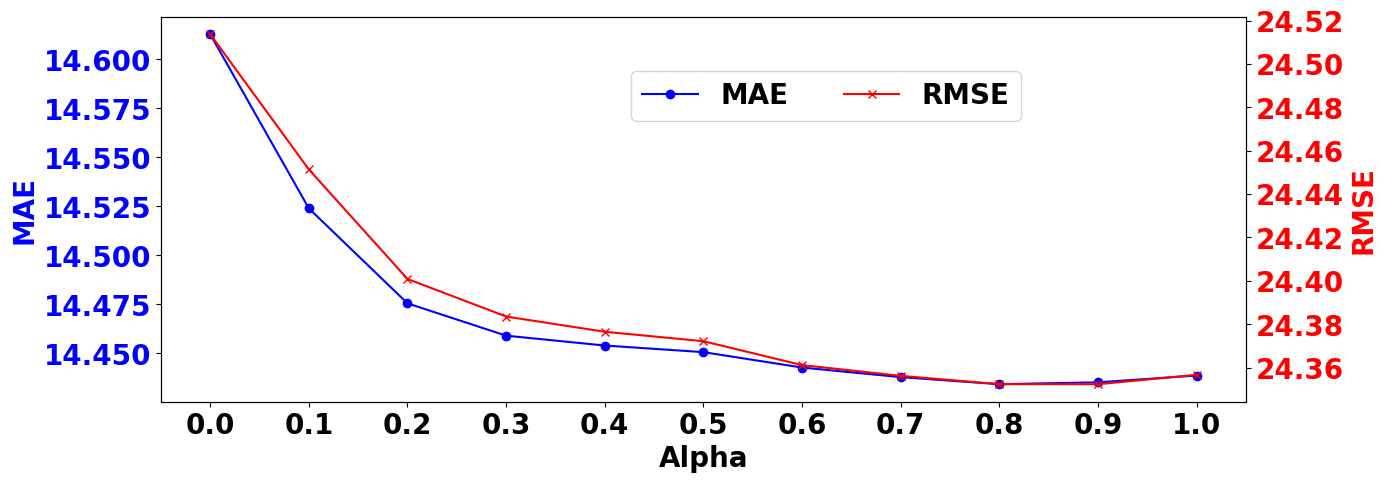
\includegraphics[width=0.8\textwidth]{figures/pems07_mae_rmse_alpha.png        }
        \caption{Distribution and mean values of predictions vs. actual truths across initial batch iterations in PEMS04.}
    \end{figure}
\end{frame}

\begin{frame}
    \frametitle{Overview of ProGen Performance}
    \framesubtitle{Random Test Runs}

    \begin{figure}[ht]
        \centering
        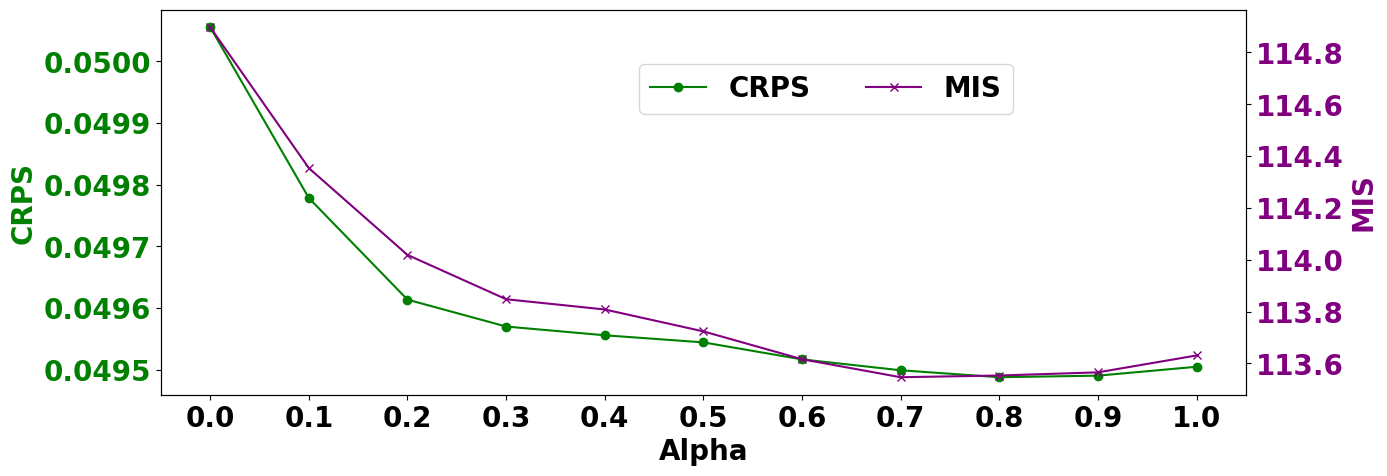
\includegraphics[width=0.8\textwidth]{figures/pems07_crps_mis_alpha.png        }
        \caption{Distribution and mean values of predictions vs. actual truths across initial batch iterations in PEMS04.}
    \end{figure}
\end{frame}



% % % % % % % % % % % % % % % % % % % % % % % % % % % % % % % % % % % %
% % % % % % % % % % % % % % % % % % % % % % % % % % % % % % % % % % % %
% % % % % % % % % % % % % % % % % % % % % % % % % % % % % % % % % % % %
% % % % % % % % % % % % % % % % % % % % % % % % % % % % % % % % % % % %
% % % % % % % % % % % % % % % % % % % % % % % % % % % % % % % % % % % %
% % % % % % % % % % % % % % % % % % % % % % % % % % % % % % % % % % % %
% % % % % % % % % % % % % % % % % % % % % % % % % % % % % % % % % % % %
% % % % % % % % % % % % % % % % % % % % % % % % % % % % % % % % % % % %

\appendix % to start a separate page numbering

\section*{Bibliography}
\begin{frame}[allowframebreaks]
    \textbf{References}
    \printbibliography
\end{frame}


{ % all template changes are local to this group.
\setbeamertemplate{navigation symbols}{}
\begin{frame}<article:0>[plain,noframenumbering]
    \begin{tikzpicture}[remember picture,overlay]
        \node[at=(current page.center)] {
            
\includegraphics[
                width=\paperwidth,
                height=\paperheight]{figures/ThankYouPage.png}
        };
    \end{tikzpicture}
    % \begin{tikzpicture}[remember picture,overlay]
    %     \node[at=(current page.center)] {
    %         
\includegraphics[keepaspectratio,
    %             width=0.65\paperwidth,
    %             height=\paperheight]{figures/ThankYouPage.png}
    %     };
    % \end{tikzpicture}
\end{frame}
}

\end{document}
